\documentclass[
  man,
  floatsintext,
  longtable,
  nolmodern,
  notxfonts,
  notimes,
  mask,
  colorlinks=true,linkcolor=blue,citecolor=blue,urlcolor=blue]{apa7}

\usepackage{amsmath}
\usepackage{amssymb}



\usepackage[bidi=default]{babel}
\babelprovide[main,import]{english}


% get rid of language-specific shorthands (see #6817):
\let\LanguageShortHands\languageshorthands
\def\languageshorthands#1{}

\RequirePackage{longtable}
\RequirePackage{threeparttablex}

\makeatletter
\renewcommand{\paragraph}{\@startsection{paragraph}{4}{\parindent}%
	{0\baselineskip \@plus 0.2ex \@minus 0.2ex}%
	{-.5em}%
	{\normalfont\normalsize\bfseries\typesectitle}}

\renewcommand{\subparagraph}[1]{\@startsection{subparagraph}{5}{0.5em}%
	{0\baselineskip \@plus 0.2ex \@minus 0.2ex}%
	{-\z@\relax}%
	{\normalfont\normalsize\bfseries\itshape\hspace{\parindent}{#1}\textit{\addperi}}{\relax}}
\makeatother




\usepackage{longtable, booktabs, multirow, multicol, colortbl, hhline, caption, array, float, xpatch}
\usepackage{subcaption}
\renewcommand\thesubfigure{\Alph{subfigure}}
\setcounter{topnumber}{2}
\setcounter{bottomnumber}{2}
\setcounter{totalnumber}{4}
\renewcommand{\topfraction}{0.85}
\renewcommand{\bottomfraction}{0.85}
\renewcommand{\textfraction}{0.15}
\renewcommand{\floatpagefraction}{0.7}

\usepackage{tcolorbox}
\tcbuselibrary{listings,theorems, breakable, skins}
\usepackage{fontawesome5}

\definecolor{quarto-callout-color}{HTML}{909090}
\definecolor{quarto-callout-note-color}{HTML}{0758E5}
\definecolor{quarto-callout-important-color}{HTML}{CC1914}
\definecolor{quarto-callout-warning-color}{HTML}{EB9113}
\definecolor{quarto-callout-tip-color}{HTML}{00A047}
\definecolor{quarto-callout-caution-color}{HTML}{FC5300}
\definecolor{quarto-callout-color-frame}{HTML}{ACACAC}
\definecolor{quarto-callout-note-color-frame}{HTML}{4582EC}
\definecolor{quarto-callout-important-color-frame}{HTML}{D9534F}
\definecolor{quarto-callout-warning-color-frame}{HTML}{F0AD4E}
\definecolor{quarto-callout-tip-color-frame}{HTML}{02B875}
\definecolor{quarto-callout-caution-color-frame}{HTML}{FD7E14}

%\newlength\Oldarrayrulewidth
%\newlength\Oldtabcolsep


\usepackage{hyperref}




\providecommand{\tightlist}{%
  \setlength{\itemsep}{0pt}\setlength{\parskip}{0pt}}
\usepackage{longtable,booktabs,array}
\usepackage{calc} % for calculating minipage widths
% Correct order of tables after \paragraph or \subparagraph
\usepackage{etoolbox}
\makeatletter
\patchcmd\longtable{\par}{\if@noskipsec\mbox{}\fi\par}{}{}
\makeatother
% Allow footnotes in longtable head/foot
\IfFileExists{footnotehyper.sty}{\usepackage{footnotehyper}}{\usepackage{footnote}}
\makesavenoteenv{longtable}

\usepackage{graphicx}
\makeatletter
\newsavebox\pandoc@box
\newcommand*\pandocbounded[1]{% scales image to fit in text height/width
  \sbox\pandoc@box{#1}%
  \Gscale@div\@tempa{\textheight}{\dimexpr\ht\pandoc@box+\dp\pandoc@box\relax}%
  \Gscale@div\@tempb{\linewidth}{\wd\pandoc@box}%
  \ifdim\@tempb\p@<\@tempa\p@\let\@tempa\@tempb\fi% select the smaller of both
  \ifdim\@tempa\p@<\p@\scalebox{\@tempa}{\usebox\pandoc@box}%
  \else\usebox{\pandoc@box}%
  \fi%
}
% Set default figure placement to htbp
\def\fps@figure{htbp}
\makeatother


% definitions for citeproc citations
\NewDocumentCommand\citeproctext{}{}
\NewDocumentCommand\citeproc{mm}{%
  \begingroup\def\citeproctext{#2}\cite{#1}\endgroup}
\makeatletter
 % allow citations to break across lines
 \let\@cite@ofmt\@firstofone
 % avoid brackets around text for \cite:
 \def\@biblabel#1{}
 \def\@cite#1#2{{#1\if@tempswa , #2\fi}}
\makeatother
\newlength{\cslhangindent}
\setlength{\cslhangindent}{1.5em}
\newlength{\csllabelwidth}
\setlength{\csllabelwidth}{3em}
\newenvironment{CSLReferences}[2] % #1 hanging-indent, #2 entry-spacing
 {\begin{list}{}{%
  \setlength{\itemindent}{0pt}
  \setlength{\leftmargin}{0pt}
  \setlength{\parsep}{0pt}
  % turn on hanging indent if param 1 is 1
  \ifodd #1
   \setlength{\leftmargin}{\cslhangindent}
   \setlength{\itemindent}{-1\cslhangindent}
  \fi
  % set entry spacing
  \setlength{\itemsep}{#2\baselineskip}}}
 {\end{list}}
\usepackage{calc}
\newcommand{\CSLBlock}[1]{\hfill\break\parbox[t]{\linewidth}{\strut\ignorespaces#1\strut}}
\newcommand{\CSLLeftMargin}[1]{\parbox[t]{\csllabelwidth}{\strut#1\strut}}
\newcommand{\CSLRightInline}[1]{\parbox[t]{\linewidth - \csllabelwidth}{\strut#1\strut}}
\newcommand{\CSLIndent}[1]{\hspace{\cslhangindent}#1}





\usepackage{newtx}

\defaultfontfeatures{Scale=MatchLowercase}
\defaultfontfeatures[\rmfamily]{Ligatures=TeX,Scale=1}





\title{The role of selective attention in value-modulated attentional
capture}


\shorttitle{THE ROLE OF SELECTIVE ATTENTION IN VMAC}


\usepackage{etoolbox}









\authorsnames[{1},{2},{3,4},{5},{1}]{Francisco Garre-Frutos,Miguel A.
Vadillo,Jan Theeuwes,Dirk Van Moorselaar,Juan Lupiáñez}







\authorsaffiliations{
{Department of Experimental Psychology and Mind, Brain, and Behavior
Research Center (CIMCYC), University of Granada, Granada,
Spain},{Department of Basic Psychology, Autonomous University of Madrid,
Madrid, Spain},{Institute Brain and Behavior Amsterdam, Department of
Experimental and Applied Psychology, Vrije Universiteit Amsterdam,
Amsterdam, the Netherlands},{William James Center for Research,
ISPA-Instituto Universitario, Lisbon, Portugal},{Faculty of Social and
Behavioral Sciences, Experimental Psychology, Helmholtz Institute,
Utrecht University, Utrecht, the Netherlands}}




\leftheader{Garre-Frutos, Vadillo, Theeuwes, Moorselaar and Lupiáñez}



\abstract{Stimuli that reliably predict reward can increase their
capacity to capture attention. This Value‑Modulated Attentional Capture
(VMAC) is typically viewed as independent of task goals or physical
salience, arising from Pavlovian learning. However, recent evidence
suggests that the awareness of the stimulus‑reward contingency may be
necessary during the acquisition of such attentional biases, although
the underlying mechanism remains unclear. One possibility is that
awareness mediates the learning process of VMAC by directing selective
attention toward the reward-predictive feature. The present
preregistered study tested whether reward‑related attentional biases
arise primarily from such selective attention, independently of
awareness. Participants performed a visual search task in which one of
two singleton distractors---one predicting high reward, the other low
reward---appeared on a subset of trials. Selective attention to the
reward‑predictive feature (distractor color) was manipulated between
groups: In some trials, one group reported the distractor's color, while
the other group reported an irrelevant feature (its location).
Otherwise, the stimulus--reward contingencies remained identical for
both groups. VMAC, as measured by slower response times for the
high‑value compared to the low‑value distractor, emerged only in the
group that reported the color. Critically, the previous result cannot be
explained by individual differences in awareness. These findings
demonstrate a causal role of selective attention in the acquisition of
reward-related attentional biases. }

\keywords{attentional capture, learning, reward, selective
attention, awareness}

\authornote{\par{\addORCIDlink{Francisco
Garre-Frutos}{0000-0001-5052-066X}}\par{\addORCIDlink{Miguel A.
Vadillo}{0000-0001-8421-816X}}\par{\addORCIDlink{Jan
Theeuwes}{0000-0002-5849-7721}}\par{\addORCIDlink{Dirk Van
Moorselaar}{0000-0002-0491-1317}}\par{\addORCIDlink{Juan
Lupiáñez}{0000-0001-6157-9894}} 

\par{Hypothesis, design and data analysis for the present study were
preregistered before data collection at
\url{https://osf.io/f3bm8}.       Author roles were classified using the
Contributor Role Taxonomy (CRediT;
\href{https://credit.niso.org}{credit.niso.org}) as follows:  Francisco
Garre-Frutos:   conceptualization, data curation, formal
Analysis, investigation, methodology, resources, Validation, software, visualization, writing
- original draft, writing - review \& editing; Miguel A.
Vadillo:   conceptualization, funding acquisition, project
administration, supervision, writing - review \& editing; Jan
Theeuwes:   conceptualization, funding acquisition, project
administration, supervision, writing - review \& editing; Dirk Van
Moorselaar:   conceptualization, funding
acquisition, supervision, writing - review \& editing; Juan
Lupiáñez:   Conceptualization, Funding acquisition, project
administration, Supervision, Writing - review \& editing}
\par{Correspondence concerning this article should be addressed
to Francisco
Garre-Frutos, Email: \href{mailto:fgfrutos@ugr.es}{fgfrutos@ugr.es}}
}

\makeatletter
\let\endoldlt\endlongtable
\def\endlongtable{
\hline
\endoldlt
}
\makeatother

\urlstyle{same}



% Restaurar sangría APA al suprimir la title page
\usepackage{indentfirst}        % indentar también el primer párrafo tras sección
\setlength{\parindent}{0.5in}   % sangría APA
\setlength{\parskip}{0pt}       % sin espacio entre párrafos
\makeatletter
\@ifpackageloaded{caption}{}{\usepackage{caption}}
\AtBeginDocument{%
\ifdefined\contentsname
  \renewcommand*\contentsname{Table of contents}
\else
  \newcommand\contentsname{Table of contents}
\fi
\ifdefined\listfigurename
  \renewcommand*\listfigurename{List of Figures}
\else
  \newcommand\listfigurename{List of Figures}
\fi
\ifdefined\listtablename
  \renewcommand*\listtablename{List of Tables}
\else
  \newcommand\listtablename{List of Tables}
\fi
\ifdefined\figurename
  \renewcommand*\figurename{Figure}
\else
  \newcommand\figurename{Figure}
\fi
\ifdefined\tablename
  \renewcommand*\tablename{Table}
\else
  \newcommand\tablename{Table}
\fi
}
\@ifpackageloaded{float}{}{\usepackage{float}}
\floatstyle{ruled}
\@ifundefined{c@chapter}{\newfloat{codelisting}{h}{lop}}{\newfloat{codelisting}{h}{lop}[chapter]}
\floatname{codelisting}{Listing}
\newcommand*\listoflistings{\listof{codelisting}{List of Listings}}
\makeatother
\makeatletter
\makeatother
\makeatletter
\@ifpackageloaded{caption}{}{\usepackage{caption}}
\@ifpackageloaded{subcaption}{}{\usepackage{subcaption}}
\makeatother

% From https://tex.stackexchange.com/a/645996/211326
%%% apa7 doesn't want to add appendix section titles in the toc
%%% let's make it do it
\makeatletter
\xpatchcmd{\appendix}
  {\par}
  {\addcontentsline{toc}{section}{\@currentlabelname}\par}
  {}{}
\makeatother

%% Disable longtable counter
%% https://tex.stackexchange.com/a/248395/211326

\usepackage{etoolbox}

\makeatletter
\patchcmd{\LT@caption}
  {\bgroup}
  {\bgroup\global\LTpatch@captiontrue}
  {}{}
\patchcmd{\longtable}
  {\par}
  {\par\global\LTpatch@captionfalse}
  {}{}
\apptocmd{\endlongtable}
  {\ifLTpatch@caption\else\addtocounter{table}{-1}\fi}
  {}{}
\newif\ifLTpatch@caption
\makeatother

\begin{document}


\section[Introduction]{The role of selective attention in
value-modulated attentional capture}

\setcounter{secnumdepth}{-\maxdimen} % remove section numbering

\setlength\LTleft{0pt}


\section*{Abstract}

Stimuli that reliably predict reward can increase their capacity to
capture attention. This Value‑Modulated Attentional Capture (VMAC) is
typically viewed as independent of task goals or physical salience,
arising from Pavlovian learning. However, recent evidence suggests that
the awareness of the stimulus‑reward contingency may be necessary during
the acquisition of such attentional biases, although the underlying
mechanism remains unclear. One possibility is that awareness mediates
the learning process of VMAC by directing selective attention toward the
reward-predictive feature. The present preregistered study tested
whether reward‑related attentional biases arise primarily from such
selective attention, independently of awareness. Participants performed
a visual search task in which one of two singleton distractors---one
predicting high reward, the other low reward---appeared on a subset of
trials. Selective attention to the reward‑predictive feature (distractor
color) was manipulated between groups: In some trials, one group
reported the distractor's color, while the other group reported an
irrelevant feature (its location). Otherwise, the stimulus--reward
contingencies remained identical for both groups. VMAC, as measured by
slower response times for the high‑value compared to the low‑value
distractor, emerged only in the group that reported the color.
Critically, the previous result cannot be explained by individual
differences in awareness. These findings demonstrate a causal role of
selective attention in the acquisition of reward-related attentional
biases.

\bigskip

\noindent\textit{Keywords:} attentional capture, learning, reward,
selective attention, awareness

\newpage

\section{The role of selective attention in value-modulated attentional
capture}\label{the-role-of-selective-attention-in-value-modulated-attentional-capture}

When individuals learn to associate a specific stimulus feature with
reward, this stimulus often becomes a stronger distractor in visual
search tasks (\citeproc{ref-anderson2021}{Anderson et al., 2021};
\citeproc{ref-failing2018}{Failing \& Theeuwes, 2018}). The weight of
evidence suggests that the learning process underlying this phenomenon
is Pavlovian in nature and thus depends on the history of
stimulus--reward pairings (e.g., \citeproc{ref-bucker2017}{Bucker \&
Theeuwes, 2017}; \citeproc{ref-mine2018}{Mine \& Saiki, 2018}). One of
the clearest demonstrations of this Pavlovian account is provided by Le
Pelley et al. (\citeproc{ref-lepelley2015}{2015}), who used a modified
version of the additional singleton task
(\citeproc{ref-theeuwes1992}{Theeuwes, 1992},
\citeproc{ref-theeuwes1994}{1994}). In their study, participants
searched for a target defined by one feature (shape), while a uniquely
colored distractor could appear on some trials. Critically, rewards were
contingent on the distractor's color---one color predicted a high reward
and the other low reward magnitude. With these settings, Le Pelley and
colleagues found that participants were slower to respond when the
high-reward singleton distractor was present compared with when the
low-reward singleton distractor appeared, even when slow responses led
to the omission of reward.

Once established, this value-modulated attentional capture (VMAC;
\citeproc{ref-anderson2011b}{Anderson et al., 2011a}) exhibits strong
features of automaticity. For example, it is largely independent of the
observer's goals (\citeproc{ref-anderson2011}{Anderson et al., 2011b};
\citeproc{ref-lepelley2015}{Le Pelley et al., 2015}), persists under
extinction (\citeproc{ref-garre-frutos2024}{Garre-Frutos et al., 2024};
\citeproc{ref-watson2019}{Watson, Pearson, Most, et al., 2019}), outcome
devaluation (\citeproc{ref-detommaso2017}{De Tommaso et al., 2017};
\citeproc{ref-detommaso2021}{De Tommaso \& Turatto, 2021};
\citeproc{ref-watson2022}{Watson et al., 2022}), and the mere passage of
time, with VMAC persisting weeks
(\citeproc{ref-anderson2019_testretest}{Anderson \& Kim, 2019})---and
even over a year (\citeproc{ref-anderson2013}{Anderson \& Yantis,
2013})---after the original learning episodes. Furthermore, VMAC is
still observed in conditions where attending to the reward-predictive
distractor is clearly counterproductive, such as when gazing at the
distractor leads to the omission of a potential reward
(\citeproc{ref-failing2015}{Failing et al., 2015};
\citeproc{ref-pearson2016}{Pearson et al., 2016}). Indeed, even when
participants actively try to prevent capture by the high-value
distractor (\citeproc{ref-pearson2020}{Pearson \& Le Pelley, 2020},
\citeproc{ref-pearson2021}{2021}), they still attend to it despite being
fully aware of the omission schedule (\citeproc{ref-pearson2015}{Pearson
et al., 2015}). Similar conclusions are often drawn about how learning
unfolds, as it is frequently assumed that learning can occur implicitly
(e.g., \citeproc{ref-anderson2016}{Anderson, 2016};
\citeproc{ref-anderson2021}{Anderson et al., 2021};
\citeproc{ref-failing2018}{Failing \& Theeuwes, 2018}). For instance,
whereas early paradigms to study VMAC established feature--reward
associations in a separate training stage where the reward-predictive
feature is task-relevant (\citeproc{ref-anderson2011}{Anderson et al.,
2011b}), subsequent research has shown that VMAC can be acquired even
when the reward-predictive feature is never task-relevant
(\citeproc{ref-mine2015}{Mine \& Saiki, 2015},
\citeproc{ref-mine2018}{2018}), response-independent
(\citeproc{ref-bucker2017}{Bucker \& Theeuwes, 2017},
\citeproc{ref-bucker2018}{2018}), or even detrimental for performance,
as in the paradigm developed by Le Pelley et al.
(\citeproc{ref-lepelley2015}{2015}).

Further support for an implicit learning account comes from reports
showing that participants often fail to identify the correct
feature-reward contingency (\citeproc{ref-anderson2015}{Anderson, 2015};
\citeproc{ref-anderson2013}{Anderson \& Yantis, 2013};
\citeproc{ref-gregoire2019}{Grégoire \& Anderson, 2019};
\citeproc{ref-theeuwes2012}{Theeuwes \& Belopolsky, 2012}), and
sometimes VMAC is observed even among those classified as ``unaware''
(\citeproc{ref-bourgeois2017}{Bourgeois et al., 2017};
\citeproc{ref-gregoire2021}{Grégoire et al., 2021};
\citeproc{ref-gregoire2019}{Grégoire \& Anderson, 2019};
\citeproc{ref-lepelley2015}{Le Pelley et al., 2015}). However, this
evidence is not as clear-cut as it may seem: other studies have found
that only participants aware of the association show VMAC
(\citeproc{ref-failing2017}{Failing \& Theeuwes, 2017};
\citeproc{ref-garre-frutos2025a}{Garre-Frutos, Lupiáñez, et al., 2025};
\citeproc{ref-lepelley2017}{Le Pelley et al., 2017};
\citeproc{ref-meyer2020}{Meyer et al., 2020}). An interesting case is
the study by Failing and Theeuwes (\citeproc{ref-failing2017}{2017}),
who conducted six experiments on the boundary conditions of VMAC. They
used a procedure similar to Le Pelley et al.
(\citeproc{ref-lepelley2015}{2015}), but the reward-predictive color
distractors were not singletons; instead, they were presented among
other colored distractors (e.g., \citeproc{ref-anderson2011}{Anderson et
al., 2011b}). Importantly, Failing and Theeuwes
(\citeproc{ref-failing2017}{2017}) instructed participants about the
color--reward contingencies in all but the last two experiments. In
Experiment 5, after four successful replications of the typical VMAC
effect, they failed to replicate it when participants were not informed
about the contingencies. In Experiment 6, they tried to facilitate
learning by reducing the number of distractor colors, and showed that
only participants who correctly identified the feature--reward
contingencies exhibited a VMAC effect.

While these findings might seem to imply that awareness is necessary for
learning, Failing and Theeuwes (\citeproc{ref-failing2017}{2017}) argued
that reducing the number of distractor colors may have merely
facilitated selective attention to the reward-predictive feature,
thereby enhancing learning. However, given that VMAC emerged only among
participants classified as aware, and selective attention was not
manipulated, such a conclusion is not warranted. A subsequent study by
Garre-Frutos, Lupiáñez, et al. (\citeproc{ref-garre-frutos2025a}{2025})
offered a more direct test: when instructions about the contingencies
were manipulated between groups, only instructed participants showed
evidence of learning. Crucially, because in Garre-Frutos, Lupiáñez, et
al. (\citeproc{ref-garre-frutos2025a}{2025}) the reward-predictive
feature was always a salient singleton distractor, selective attention
alone cannot explain the results, which suggest that awareness should
play a direct role in learning.

Viewed together, this body of evidence may appear contradictory, but it
is well established that human Pavlovian learning is strongly affected
by instructions and awareness of the contingencies
(\citeproc{ref-lovibond2011}{Lovibond et al., 2011};
\citeproc{ref-lovibond2002}{Lovibond \& Shanks, 2002};
\citeproc{ref-mertens2016}{Mertens et al., 2016};
\citeproc{ref-mertens2020}{Mertens \& Engelhard, 2020};
\citeproc{ref-weidemann2016}{Weidemann et al., 2016}). Some theoretical
accounts even propose that Pavlovian learning could be entirely
propositional (\citeproc{ref-mitchell2009}{Mitchell et al., 2009}),
making awareness a necessary condition. Still, while VMAC is a clear
example of how learning shapes attentional control, the relationship is
not one-way: attention also plays a crucial role in learning
(\citeproc{ref-mackintosh1975}{Mackintosh, 1975};
\citeproc{ref-niv2015}{Niv et al., 2015};
\citeproc{ref-pearce1980}{Pearce \& Hall, 1980}). Hence, the
interpretation raised by Failing and Theeuwes
(\citeproc{ref-failing2017}{2017}) is not unreasonable, in that learning
may depend on the kind of attention directed toward the predictive
feature (\citeproc{ref-jimuxe9nez1999}{Jiménez \& Méndez, 1999}).
Indeed, a similar result is common in other learned attentional biases,
such as visual statistical learning, where selective spatial attention
to predictive information is widely considered necessary for learning to
occur (\citeproc{ref-duncan2024}{Duncan et al., 2024};
\citeproc{ref-golan2024}{Golan et al., 2024};
\citeproc{ref-jiang2001}{Jiang \& Chun, 2001};
\citeproc{ref-vadillo2020}{Vadillo et al., 2020};
\citeproc{ref-vadillo2024}{Vadillo et al., 2024}).

A parsimonious alternative account is that awareness may influence
learning in VMAC indirectly by encouraging selective attention toward
the specific reward-predictive feature of the salient distractor. For
instance, although distractors in the additional singleton task capture
attention (\citeproc{ref-theeuwes1992}{Theeuwes, 1992},
\citeproc{ref-theeuwes1994}{1994}), participants are never explicitly
required to selectively attend to any specific singleton feature, either
location, shape, or color, as it is not directly task-relevant. In
Garre-Frutos, Lupiáñez, et al. (\citeproc{ref-garre-frutos2025a}{2025}),
instructions (and awareness) about stimulus--reward contingencies might
direct attention specifically toward the reward-associated feature,
potentially making such selective attention both necessary and
sufficient for learning. If selective attention is crucial, any
manipulation compelling participants to attend to the reward-associated
feature (color) rather than reward-irrelevant features (e.g., location)
should elicit the learning of VMAC, independently of awareness.

\subsection{The Present Study}\label{the-present-study}

This preregistered study tested the causal role of selective attention
in the learning process underlying VMAC. We followed the general
procedure of Garre-Frutos, Lupiáñez, et al.
(\citeproc{ref-garre-frutos2025a}{2025}), but instead of manipulating
instructions we added a concurrent task designed to direct selective
attention to distinct distractor dimensions. In a between-participants
manipulation, one group was asked to report the color of the singleton
distractor and the other reported its location (cf.
\citeproc{ref-gao2020}{Gao \& Theeuwes, 2020}). This design contrasted
attention to a reward-associated, task-irrelevant feature (color) with
attention to a reward-irrelevant feature (location), without informing
participants of the color--reward association (conceptually similar to
\citeproc{ref-jimuxe9nez1999}{Jiménez \& Méndez, 1999}).

We hypothesized a dissociation in VMAC based on the concurrent task
(color vs.~location). We predicted that only the color-report group
would show a VMAC effect, and that this effect would be independent of
individual differences in awareness. Specifically, we expected:

\begin{itemize}
\item
  \textbf{H1:} Replication of the typical attentional-capture effect in
  the additional-singleton task.
\item
  \textbf{H2:}

  \begin{itemize}
  \item
    \textbf{H2\textsubscript{1}:} The VMAC effect would be significantly
    larger in the color group than in the location group.
  \item
    \textbf{H2\textsubscript{2}:} The VMAC effect would be observed only
    among participants who selectively attend to color.
  \end{itemize}
\item
  \textbf{H3:} Between-group differences in VMAC (H2) would not be
  explained by individual differences in awareness.
\end{itemize}

\section{Methods}\label{methods}

\subsection{Participants}\label{participants}

We performed a simulation-based power analysis (fully reported in the
preregistration; \url{https://osf.io/f3bm8}) for the critical Group
(color vs.~location) \(\times\) Distractor (high- vs.~low-value)
interaction, based on a similar effect from the linear mixed model (LMM)
reported in Garre-Frutos, Lupiáñez, et al.
(\citeproc{ref-garre-frutos2025a}{2025}). Specifically, in Experiment 2,
the authors observed a significant interaction between Group
(instructions vs.~no instructions about the contingencies) and
Distractor (high- vs.~low-value) on response times (RTs), with only the
instructed group showing a significant VMAC effect. Given that the
present study is an extension of the same results, in similar settings
and conditions, we used the same effect size to estimate the required
sample size for 80\% power to detect the critical interaction in our
design. Importantly, given resource and time constraints for data
collection, we preregistered two decisions to maximize power: (1) we
excluded trials from the first block of the visual search task, as VMAC
is typically not observed in this block
(\citeproc{ref-garre-frutos2024}{Garre-Frutos et al., 2024};
\citeproc{ref-garre-frutos2025a}{Garre-Frutos, Lupiáñez, et al., 2025};
\citeproc{ref-garre-frutos2025b}{Garre-Frutos, Ariza, et al., 2025});
and (2) given that we have our hypothesis about the direction of the
effect, we used a one-tailed test (i.e., higher VMAC for the group
tasked to report the color vs.~location of the distractor) for the
critical interaction, as specified in the preregistration, and following
our hypotheses (H2\textsubscript{1}). Power was estimated using R
(version 4.3.1; \citeproc{ref-r_ref}{R Core Team, 2023}) and the
\emph{simr} package (\citeproc{ref-simr}{Green \& MacLeod, 2016}).
Simulations indicated that 70 participants per group would yield 84\%
power (\(\alpha = .05\)).

To account for potential exclusions, we collected data from 80
participants per group (\emph{N} = 160). Following the preregistered
protocol, seven participants were excluded due to low accuracy
(\textless{} 70\%), RTs deviating ±3 SD from the group mean, or poor
performance in the concurrent task\footnote{As described below,
  participants in the visual search task completed 288 trials, but were
  required to report the distractor's location or color on only 12--24
  trials (randomly across participants). Rather than setting a fixed
  accuracy cutoff, we included only those participants performing above
  chance on the concurrent task to ensure appropriate performance. As
  preregistered, this threshold was determined using a binomial test
  with \(p = 0.5\). For example, a participant who completed 12 report
  trials would need at least 10 correct responses (\(p = .036\)) to meet
  the threshold, whereas a participant with 18 trials would require at
  least 14 correct responses (\(p = .031\)). Thus, the accuracy cutoff
  varies between 75\% and 83\%, depending on the number of report trials
  completed.}. The final sample included 153 participants
(\(n_{\text{color}} = 77\), \(n_{\text{location}} = 76\); 117
self-identified as women; \(M_{\text{age}} = 21.4\), \(SD = 4.2\)).

\subsection{Stimuli, Materials, and
Procedure}\label{stimuli-materials-and-procedure}

The materials and procedure were based on Garre-Frutos, Lupiáñez, et al.
(\citeproc{ref-garre-frutos2025a}{2025}). The study was conducted
online, consistent with prior work using this task
(\citeproc{ref-albertella2019}{Albertella et al., 2019};
\citeproc{ref-albertella2020}{Albertella et al., 2020};
\citeproc{ref-garre-frutos2024}{Garre-Frutos et al., 2024};
\citeproc{ref-garre-frutos2025a}{Garre-Frutos, Lupiáñez, et al., 2025};
\citeproc{ref-gonzalez2025}{González et al., 2025};
\citeproc{ref-lepelley2022}{Le Pelley et al., 2022};
\citeproc{ref-liu2021}{Liu et al., 2021};
\citeproc{ref-watson2020}{Watson et al., 2020}). The task was programmed
in jsPsych (\citeproc{ref-leeuw2023}{Leeuw et al., 2023}) and hosted on
JATOS (\citeproc{ref-lange2015}{Lange et al., 2015}). To control for
differences in participants' distance from the screen, we scaled
stimulus size to screen distance using the virtual chinrest developed by
Q. Li et al. (\citeproc{ref-li2020}{2020}). Before starting the main
task, participants underwent a calibration procedure to estimate screen
distance. They adjusted the size of a rectangle on their screen to match
a standard-sized object (e.g., a credit card or driver's license). Then,
they performed a blind spot measurement by covering their right eye and
focusing their left eye on a central placeholder while a red circle
moved leftward, pressing the space bar when the circle disappeared. This
process was repeated five times, and the average was used to estimate
screen distance.

As depicted in Figure~\ref{fig-1}, each trial started with a central
fixation cross, followed by a search display containing six shapes (2.3°
× 2.3° visual angle) arranged evenly around an imaginary circle with a
diameter of 10.1°. The target was a diamond-shaped stimulus containing a
line segment oriented either horizontally or vertically, and the
non-targets were five circles each containing a line segment tilted 45°
to the left or right. On most trials, one of the circles appeared as a
uniquely colored singleton distractor (orange/blue or pink/green,
counterbalanced), which could be either a high- or low-value color,
counterbalanced within each pair. The remaining shapes were gray. The
positions of the target and distractor varied randomly in each trial.
Participants were instructed to find and report the orientation of the
line segment inside the diamond as quickly as possible by pressing the
\textless b\textgreater{} key for horizontal or the
\textless j\textgreater{} key for vertical. The search display remained
on screen until the participant responded or 2000 ms had elapsed.
Feedback indicating points won or lost was displayed for 700 ms, and the
inter-trial interval was 1200 ms.

\begin{figure}[htpb]

{\caption{{Schematic representation of the task.}{\label{fig-1}}}}

\begin{center}
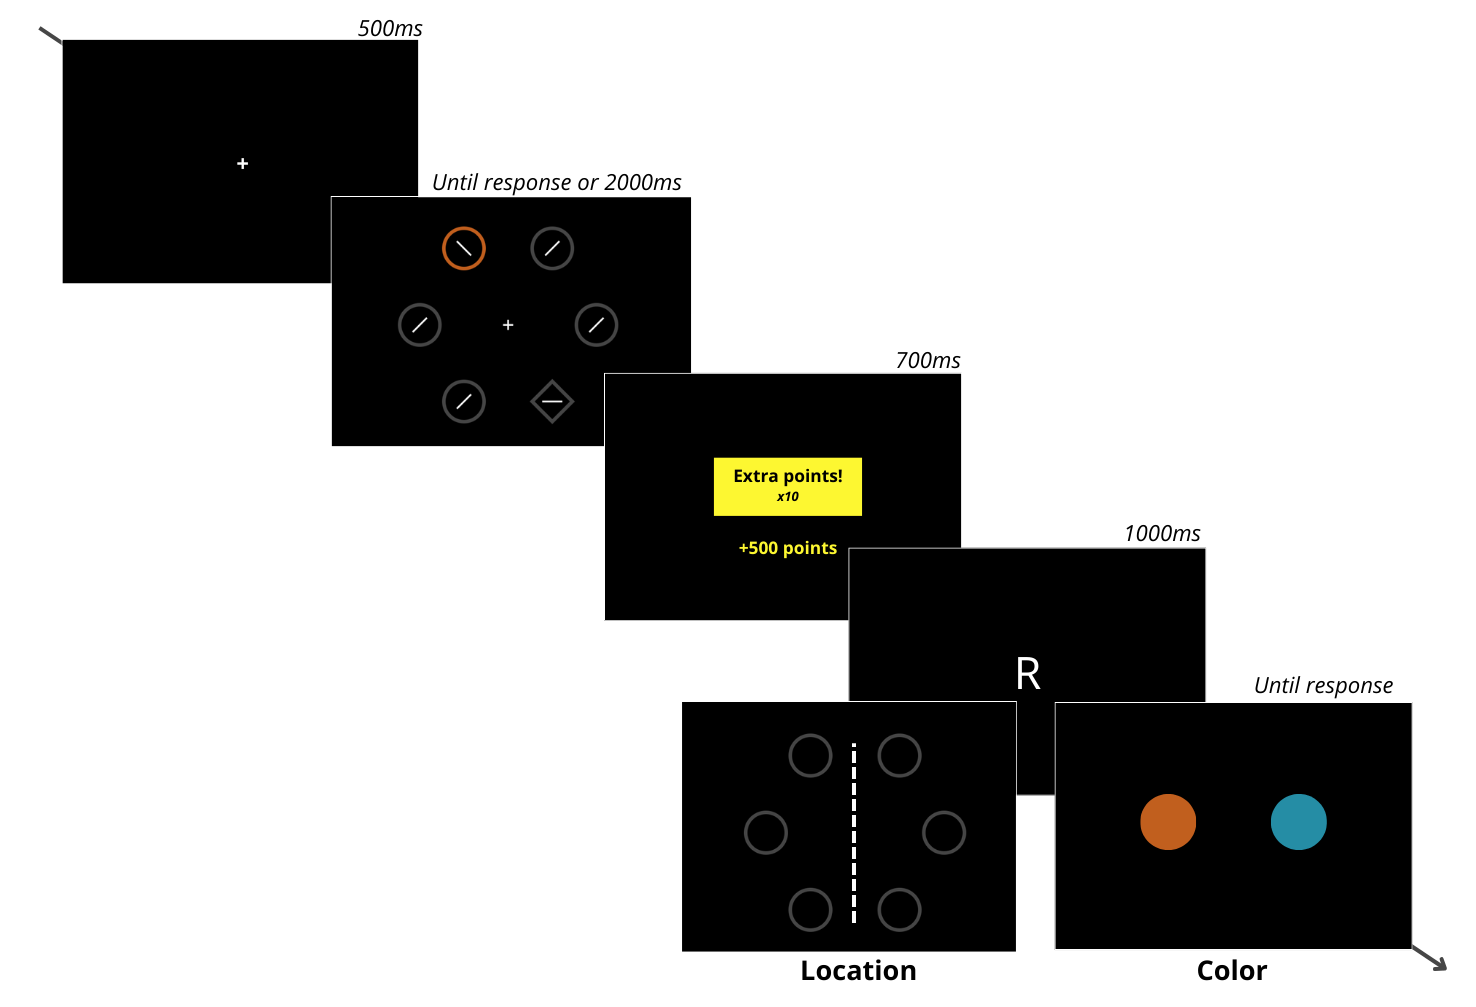
\includegraphics[width=4.92in,height=\textheight,keepaspectratio]{pre_registation/figure_3.png}
\end{center}

{\noindent \emph{Note.} Example of the sequence of events in the
experimental task. Participants could earn points based on performance,
and when a high-value singleton appeared in the display, points were
multiplied by 10 (a bonus trial). In some trials, participants were
presented with the letter `R', which signaled that participants had to
report the color or the location (as a function of the assigned group)
of the distractor in the preceding trial.}

\end{figure}

The task consisted of six blocks of 48 trials (20 high-value singleton
trials, 20 low-value singleton trials, and 8 distractor-absent trials).
Occasionally, participants encountered report trials, indicated by an
``R'' presented for 1000 ms immediately after the feedback display.
Report trials occurred infrequently (two to four per block) with the
constraint that at least one appeared in each half of the block; they
were restricted to distractor-present trials. On report trials,
participants indicated either the side (left or right) of the display on
which the distractor had appeared (report location group) or the
distractor's color (report color group). In both groups, responses were
made with the \textless c\textgreater{} and \textless m\textgreater{}
keys, which always corresponded to the left and right on-screen response
options, respectively\footnote{For both groups, response keys were
  always mapped to the same relative positions on the keyboard (e.g.,
  \textless c\textgreater{} = left, \textless m\textgreater{} = right).
  In the color group, either distractor color could appear on the left
  or right side of the screen during report trials (see
  Figure~\ref{fig-1}). Because the singleton distractor's position was
  randomized on every search trial, there was no systematic association
  between report responses (color or side) and distractor location. In
  other words, location and singleton color were completely independent
  in both groups.}. Correct responses in the report task earned 2000
points, whereas incorrect responses lost 2000 points; feedback on report
performance was provided at the end of each block. In the visual search
task, participants received 0.1 points for every millisecond their RTs
were below 1000 ms on low-value distractor trials, and the number of
points earned was multiplied by 10 on high-value distractor trials. No
points were earned for RTs exceeding 1000 ms, and incorrect responses
resulted in a loss of points equivalent to the potential gain for that
trial. With this manipulation, participants distracted by the high-value
singleton would acquire significantly fewer points, as the number of
points earned in a given trial is directly proportional to performance.

After the calibration phase, participants first completed 20 practice
trials without any singleton distractor to familiarize themselves with
the task. They then performed 10 trials with both the visual search task
and the report task (after every trial). In this practice stage, the
search display was presented for 10 seconds. After this, participants
performed 20 additional trials at normal speed. Subsequently, they
entered the visual search task, where instructions emphasized that
faster and correct responses result in more points, while incorrect
responses result in point losses. Importantly, participants were not
informed about the association between the distractor color and reward
value. They were only reminded about the distractor's in relation to the
report task.

At the end of the experiment, participants completed an awareness test
to assess their knowledge of the color-reward contingencies using a
Visual Analog Scale (VAS; \citeproc{ref-Reips2008}{Reips \& Funke,
2008}), following the procedure implemented by Garre-Frutos, Lupiáñez,
et al. (\citeproc{ref-garre-frutos2025a}{2025}). They were instructed to
respond based on their impressions during the task, avoiding post-hoc
interpretations. First, participants rated the extent to which they
believed distractor color influenced the likelihood of ``bonus trials''
(contingency belief), with the scale ranging from 0 (``I don't believe
color makes any difference'') to 100 (``I believe color completely
determines the likelihood of bonus trials''). They then estimated the
relative proportion of bonus trials associated with each color
(contingency awareness). To do this, they were presented with another
VAS showing the high- and low-rated distractors with endpoints
indicating the percentage of bonus trials estimated to be associated
with each color. Participants adjusted a dot along the VAS to represent
their estimated likelihood, which updated the displayed percentages
accordingly (e.g., a position closer to the high-value color might show
a 70\% likelihood for the high-value distractor and 30\% for the
low-value singleton). After providing these ratings, participants
indicated their confidence using a confidence VAS ranging from 0 (``no
confidence'') to 100 (``very confident''). Finally, participants had the
opportunity to provide a free-form qualitative description of any
patterns they noticed in the likelihood of bonus trials; this response
was collected only for exploratory purposes.

\subsection{Data analysis}\label{data-analysis}

Unless noted otherwise, all analyses followed our preregistered plan,
including data selection criteria, significance thresholds, and the
directionality of hypotheses. Data were analyzed using R, version 4.3.1
(\citeproc{ref-r_ref}{R Core Team, 2023})\footnote{R packages:
  \emph{lme4} (\citeproc{ref-lme4}{Bates, Mächler, et al., 2015}),
  \emph{betareg} (\citeproc{ref-betareg}{Cribari-Neto \& Zeileis,
  2010}), \emph{marginaleffects}
  (\citeproc{ref-R-marginaleffects}{Arel-Bundock et al., Forthcoming}),
  and \emph{tidyverse} (\citeproc{ref-tidyverse}{Wickham et al., 2019}).}.

\subsubsection{Report task}\label{report-task}

We first analyzed performance in the report task. To that aim, we
compared the two groups on report-task accuracy by fitting a multilevel
logistic regression (\citeproc{ref-jaeger2008}{Jaeger, 2008}) with a
Group predictor and a by-participant random intercept.

\subsubsection{Visual search task}\label{visual-search-task}

The main dependent variable was RTs. We removed RTs considered outliers
(RTs \textless{} 150 or \textgreater{} 1800 ms; 0.57\%), incorrect
responses (5.53\%) and, following our power analysis, we removed all
trials from the first block. Log-transformed RTs were analyzed using an
LMM including predictors Singleton (high-value, low-value, absent
distractor), Group (color, location), and their interaction. Group was
coded using deviation coding. For Singleton, we used repeated contrasts:
one contrast for high-value vs.~low-value (VMAC effect) and another for
low-value vs.~absent (Attentional Capture effect; AC effect). This
strategy allowed us to test specific hypotheses regarding each
theoretically relevant contrast (\citeproc{ref-schad2020}{Schad et al.,
2020})\footnote{Specifically, the fixed-effects structure of the LMM had
  five coefficients: one for Group, two for Singleton (high-value
  vs.~low-value; low-value vs.~absent), and two for the interactions
  between Group and each Singleton contrast. This allowed testing
  specific hypotheses instead of an omnibus test with no direct
  theoretical relevance.}. We tested for significance using the
preregistered criteria, assuming an \(\alpha = 0.05\) and two-sided
contrast. The only exception was the interaction between Group and the
VMAC effect, for which we used a one-sided contrast reflecting our
directional hypothesis (H2\textsubscript{1}). If a significant Group
\(\times\) VMAC interaction was observed, we computed the conditional
VMAC effect for each group. The model's formula, as implemented in the
\emph{lme4} R package (\citeproc{ref-lme4}{Bates, Mächler, et al.,
2015}), was as follows:

\[ 
\log(\text{RT}) \sim \text{Group} \times \text{Singleton} + (\text{Singleton} \ | \ \text{ID})
\]

Regarding the random-effects structure, we first fit the maximum
random-effects structure justified by our design
(\citeproc{ref-barr2013}{Barr et al., 2013}), including a random slope
for the Singleton predictor. In cases of convergence problems or
singular fits, we reduced the random-effects structure
(\citeproc{ref-bates2015}{Bates, Kliegl, et al., 2015};
\citeproc{ref-matuschek2017}{Matuschek et al., 2017}), by dropping the
random slope for Singleton. Finally, because between-group comparisons
are possibly attenuated by measurement error
(\citeproc{ref-karvelis}{Karvelis \& Diaconescu, 2025};
\citeproc{ref-wiernik2020}{Wiernik \& Dahlke, 2020}; but see
\citeproc{ref-parsons2018}{Parsons, 2018}), we calculated the split-half
reliability (\citeproc{ref-parsons2021}{Parsons, 2021}) of the VMAC
effect for each group to inform potential attenuation in the critical
between-group comparison.

Finally, although we had no theoretical interest in task accuracy (which
is usually near ceiling in similar tasks;
\citeproc{ref-garre-frutos2025a}{Garre-Frutos, Lupiáñez, et al., 2025};
\citeproc{ref-garre-frutos2025b}{Garre-Frutos, Ariza, et al., 2025};
\citeproc{ref-watson2019}{Watson, Pearson, Most, et al., 2019}), we
analyzed accuracy to rule out a speed--accuracy trade-off. We fit a a
multilevel logistic regression, using the same fixed-effects structure
as in the RT LMM and the same strategy for selecting the random-effects
structure.

\subsubsection{Awareness tests}\label{awareness-tests}

Participants reported, using two VAS scales (coded 0--100), (1) their
belief in the probability of a bonus trial depending on the distractor's
color (\emph{Contingency belief}), and (2) their estimate of the
relative likelihood of receiving a bonus trial based on the distractor's
color (\emph{Contingency awareness}). Because both measures are bounded
between 0 and 100, we used beta regression
(\citeproc{ref-smithson2006}{Smithson \& Verkuilen, 2006})\footnote{As
  discussed by Smithson and Verkuilen
  (\citeproc{ref-smithson2006}{2006}), beta regression assumes known
  boundaries in the dependent variable but cannot model responses at
  those exact boundaries. Following their recommendation, we applied a
  scaling transformation to avoid boundary values:
  \(y' = [y' \cdot (N - 1) + 1/2] / N\).}, including a Group predictor
to test for mean differences across groups on each VAS.

Each VAS response included an accompanying confidence rating to assess
metacognitive validity. To examine the validity of the awareness
measures as indicators of explicit knowledge of the feature--reward
contingency, we fit the beta-regression models separately for each
group, incorporating confidence ratings as predictors. A positive
relationship between confidence and performance on the awareness
measures would support their validity. Additionally, to evaluate whether
the first awareness question predicts the second, we employed the same
beta-regression approach.

As preregistered, interpreting H2 as the causal effect of selective
attention on learning required no between-group differences in awareness
(H3). To that aim, we tested whether controlling for these individual
differences eliminated the Group \(\times\) VMAC interaction by
including the awareness response as a covariate in the RT model
described above. To simplify this model, we excluded distractor-absent
trials. Because we had two awareness measures, if these measures showed
convergent validity (e.g., contingency awareness predicts contingency
belief), we used the second contingency awareness as the covariate,
which is more similar to the measure employed by Garre-Frutos, Lupiáñez,
et al. (\citeproc{ref-garre-frutos2025a}{2025}).

\section{Results}\label{results}

\subsection{Report task}\label{report-task-1}

Accuracy was high
(\(M_{\text{Accuracy}} = 0.946, \;95\%\,\text{CI}[0.933, 0.959]\)) and
did not differ significantly between groups (\emph{p} = 0.749),
suggesting that participants performed well on the secondary task.

\subsection{Visual search task}\label{visual-search-task-1}

RTs analysis showed significant VMAC
(\(\beta_{\mathrm{VMAC}} = 0.008, \; t_{151} = 2.57, \; p = 0.011\)) and
AC (\(\beta_{\mathrm{AC}} = 0.062, \; t_{151} = 17.26, \; p < 0.001\))
effects (Figure \hyperref[fig-2]{2A}), indicating that participants were
slower in the presence of a high-
(\(M_{\mathrm{High}} = 734.2,\;95\%\,\mathrm{CI}[719.7, 748.9]\))
compared to a low-value distractor
(\(M_{\mathrm{Low}} = 728.4,\;95\%\,\mathrm{CI}[713.8, 743.3]\)), and
faster when no distractor was present
(\(M_{\mathrm{Absent}} = 684.2,\;95\%\,\mathrm{CI}[671.1, 697.6]\)).
Critically, the Group predictor interacted significantly only with VMAC
(\(\beta_{\mathrm{VMAC} \times \mathrm{Group}} = 0.006, \; t_{151} = 1.98, \; p = 0.025\)),
such that a significant VMAC effect was observed in the color group
(\(M_{\mathrm{VMAC}} = 10.4,\;95\%\,\mathrm{CI}[4.0, 16.8]\)) but not in
the location group
(\(M_{\mathrm{VMAC}} = 1.2,\;95\%\,\mathrm{CI}[-5.3, 7.6]\))\footnote{Split-half
  reliability of the VMAC effect was low
  (\(r_{\text{sb}} = 0.28, \;95\%\,\text{CI}[0.09, 0.44]\)) compared to
  previous studies using this task
  (\citeproc{ref-garre-frutos2024}{Garre-Frutos et al., 2024};
  \citeproc{ref-garre-frutos2025a}{Garre-Frutos, Lupiáñez, et al.,
  2025}), maybe because of the dual-task design. This suggests that
  between-groups differences are possibly attenuated by measurement
  error (\citeproc{ref-karvelis}{Karvelis \& Diaconescu, 2025};
  \citeproc{ref-wiernik2020}{Wiernik \& Dahlke, 2020}; but see
  \citeproc{ref-parsons2018}{Parsons, 2018}).}. No other effects reached
significance (\emph{ps} \textgreater{} 0.133).

\begin{figure}[htbp]

{\caption{{Summary of results}{\label{fig-2}}}}

\pandocbounded{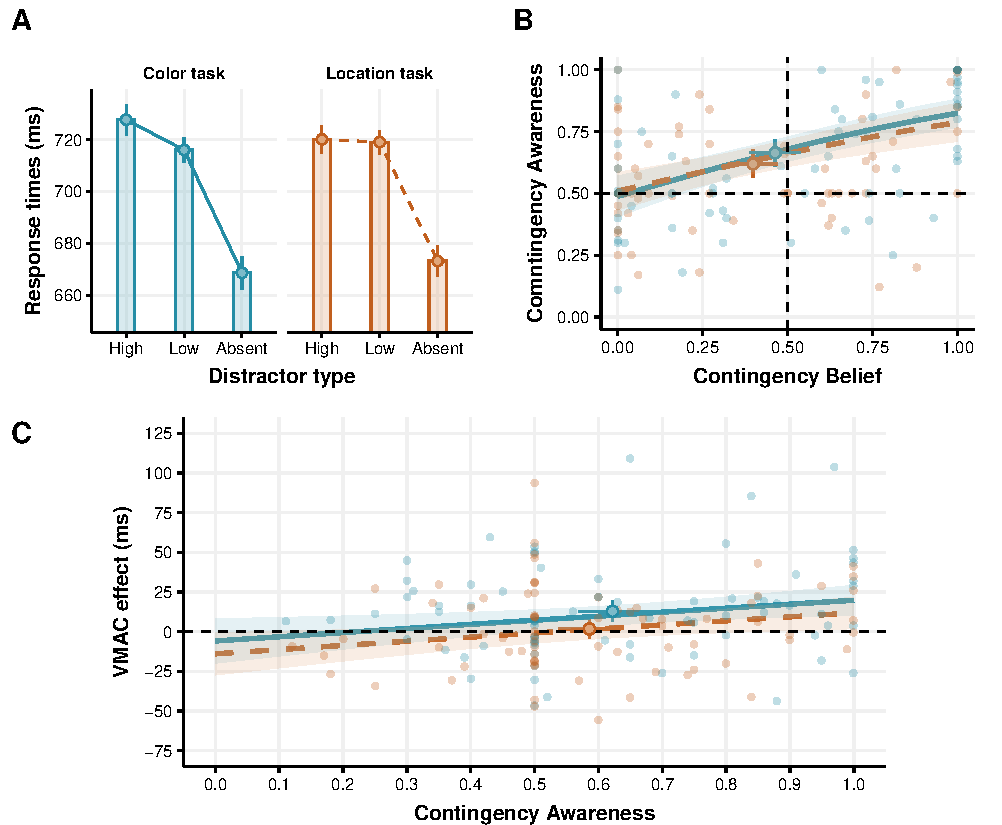
\includegraphics[keepaspectratio]{Output/plots/fig2.pdf}}

{\noindent \emph{Note.} \textbf{A}) Mean RTs in the visual search task.
Bars and dots show condition means; error bars indicate within-subject
95\% CIs (\citeproc{ref-morey2008}{Morey, 2008}). \textbf{B}) Beta
regression predictions for awareness results. Transparent dots are
individual responses; lines and shaded areas show model predictions and
95\% CIs, and solid dot points and error bars represent mean predicted
responses at the group-level. \textbf{C}) RT analysis with contingency
awareness as covariate. Transparent dots show individual VMAC scores;
lines and shaded areas depict model predictions by task and awareness
level. Solid, large dots and error bars show group means and 95\% CIs.
Note that both the selective attention manipulation and contingency
awareness have independent effects on observed VMAC scores, showing that
our results cannot be explained by individual differences in awareness.}

\end{figure}

Accuracy in the visual search task was high
(\(M_{\text{Accuracy}} = 0.953, \;95\%\,\text{CI}[0.948, 0.959]\)) and
none of the predictors reached significance (\emph{ps} \textgreater{}
0.365), indicating that the above results cannot be explained by a
speed--accuracy trade-off.

\subsection{Awareness}\label{awareness}

Neither awareness measure differed significantly between groups
(\emph{ps} \textgreater{} 0.224), and the two awareness measures were
significantly correlated (\(\beta = 0.551,\ z = 6.632,\ p < 0.001\);
Figure \hyperref[fig-2]{2B}) with no significant group differences in
this correlation (\emph{p} = 0.444). Furthermore, while contingency
awareness was positively associated with its corresponding confidence
rating (\(\beta = 0.579,\ z = 7.197,\ p < 0.001\); no group difference,
\emph{p} = 0.409), contingency belief was not (\emph{ps} \textgreater{}
0.231). Overall, these results suggest convergent validity regarding
explicit knowledge of the feature--reward contingency, particularly for
contingency awareness.

As preregistered, we repeated the analysis of RTs restricted to high-
and low-value distractor trials, including contingency awareness and its
interaction with VMAC as covariates. This analysis revealed a
significant VMAC \(\times\) Contingency Awareness interaction
(\(\beta_{\mathrm{VMAC} \times \mathrm{Awareness}} = 0.004, \; t_{151} = 2.58, \; p = 0.011\)),
indicating that VMAC was positively associated with contingency
awareness (Figure \hyperref[fig-2]{2C}). Critically, the VMAC × Group
interaction remained significant
(\(\beta_{\mathrm{VMAC} \times \mathrm{Group}} = 0.003, \; t_{151} = 1.80, \; p = 0.037\))
after controlling for individual differences in awareness\footnote{As
  preregistered, given that both awareness measures showed convergent
  validity, we used contingency awareness as the covariate (as in
  \citeproc{ref-garre-frutos2025a}{Garre-Frutos, Lupiáñez, et al.,
  2025}). However, as a (non-preregistered) robustness test, we showed
  that the results remain unchanged if we use contingency belief, or
  even if we multiply each awareness measure by its corresponding
  confidence rating (\emph{ps} \textless{} 0.031).}. Follow-up analyses
controlling by awareness revealed that the color group still showed a
significant VMAC effect
(\(M_{\mathrm{VMAC}} = 7.2,\;95\%\,\mathrm{CI}[0.6, 13.8]\)), while the
location group did not
(\(M_{\mathrm{VMAC}} = -0.9,\;95\%\,\mathrm{CI}[-7.3, 5.5]\)).
Therefore, even though the VMAC effect was modulated by awareness, the
interaction with selective attention cannot be explained away by
individual differences in awareness alone.

\section{Meta-analysis}\label{meta-analysis}

To contextualize our findings and understand their practical
implications, we performed a (non-preregistered) meta-analysis on
previous studies employing the same design and settings. Specifically,
the present task is an almost exact replication of Garre-Frutos et al.
(\citeproc{ref-garre-frutos2024}{2024}), and the present study derives
from Garre-Frutos, Lupiáñez, et al.
(\citeproc{ref-garre-frutos2025a}{2025}). We compared our results with
the standardized effect sizes observed in those studies. Additionally,
to get a sense of how effect sizes in this specific task design relate
to the overall literature, we compared our effect sizes to the
meta-analytical estimate from the study of Rusz et al.
(\citeproc{ref-rusz2020}{2020}), a meta-analysis aiming to characterize
the size of reward-driven distraction across a wide range of
experimental paradigms.

\begin{figure}[htbp]

{\caption{{Meta-analysis comparing the present results with prior
literature}{\label{fig-3}}}}

\pandocbounded{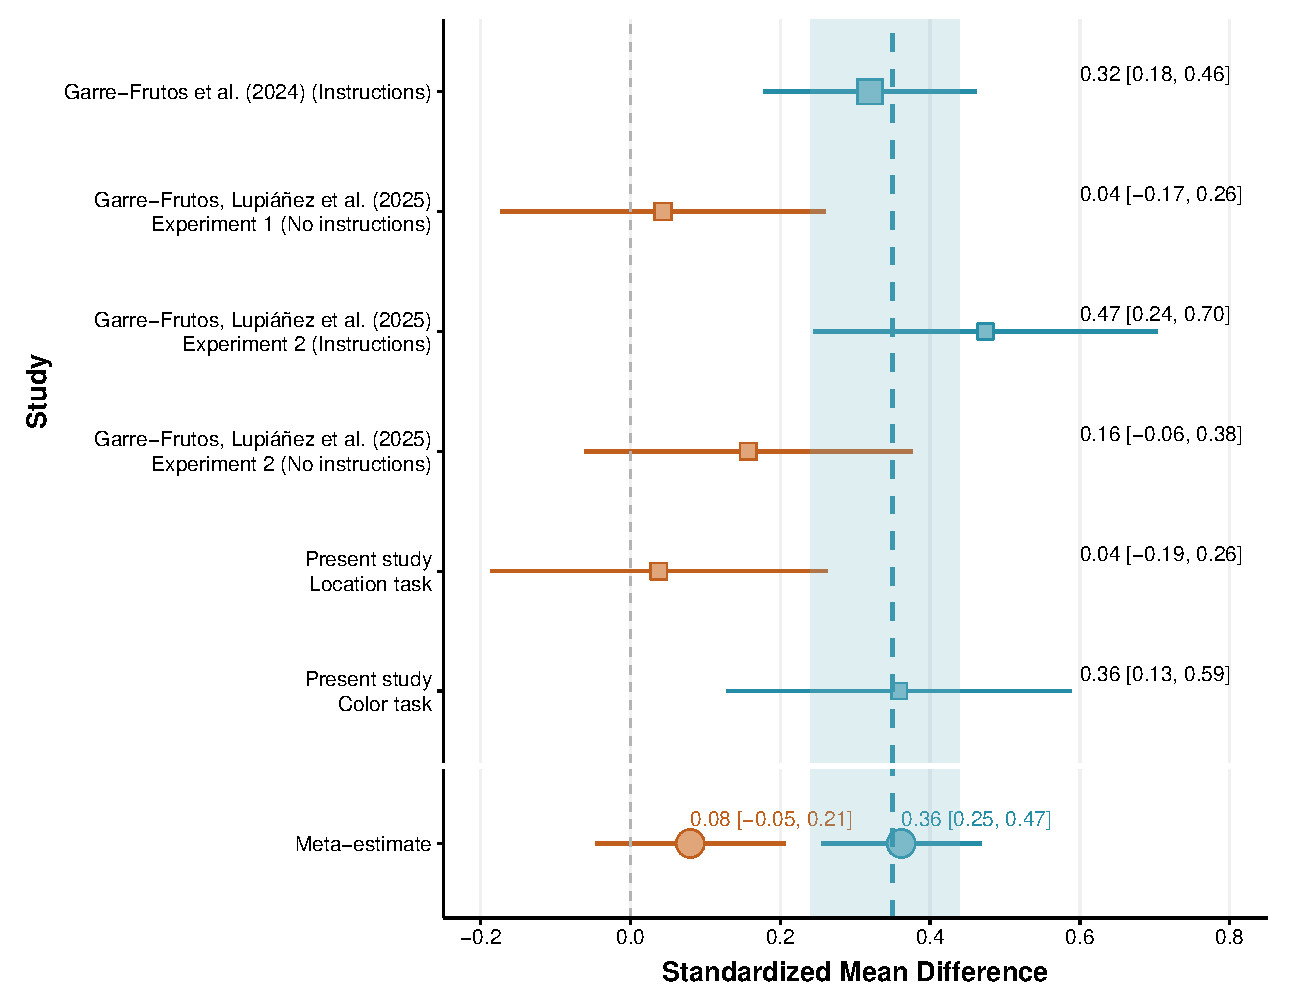
\includegraphics[keepaspectratio]{Output/plots/fig3.pdf}}

{\noindent \emph{Note.} To illustrate the conceptual similarities
between manipulating instructions and selective attention, blue
indicates that participants received instructions about the
feature-reward contingency or selectively attended to color (in the
present study). In contrast, orange means that they did not receive
instructions or selectively attended to the location (in the present
study). The blue dashed line and the shaded segments indicate the
meta-analytic estimate (Standardized Mean Difference) and the 95\% CI of
the effect of reward-driven distraction in the broader literature (0.35;
Rusz et al., 2020). Squares indicate standardized effect sizes for
individual studies, with size indicating precision and error bars
indicating CI. Results from the meta-analysis showed that the effect
size observed in the present study for the color group is perfectly
consistent with effect sizes observed in the literature and prior
studies.}

\end{figure}

Regarding the calculation of effect sizes, as in Rusz et al.
(\citeproc{ref-rusz2020}{2020}), we estimated the Standardized Mean
Difference (\emph{SMD}) for the VMAC effect as:

\[
\mathrm{SMD} \;=\; \frac{M_{\text{high}} - M_{\text{low}}}{\sqrt{SD_{\text{high}}^{2} + SD_{\text{low}}^{2} - 2r\,SD_{\text{high}}SD_{\text{low}}}}
\]

where \(M\) and \(SD\) are the condition means and standard deviations,
and \(r\) is the within-participant correlation. The sampling variance
was estimated as:

\[
V_{\mathrm{SMD}} \;=\; \frac{1}{n} + \frac{\mathrm{SMD}^{2}}{2n}.
\]

We also estimated the same meta-analytic model using raw differences in
RTs to facilitate interpretation of effect sizes within this specific
task design. We estimated the sampling variance for raw RTs as:

\[
V_{\mathrm{Raw}} \;=\; \frac{SD_{\text{high}}^{2} + SD_{\text{low}}^{2} - 2r\,SD_{\text{high}}SD_{\text{low}}}{n}.
\]

We fitted a random-effects model using the \emph{metafor} package
(\citeproc{ref-metafor}{Viechtbauer, 2010}), including a moderator
coding whether participants were encouraged to attend to the
reward-predictive feature---via (or lack of) instructions in prior
studies (\citeproc{ref-garre-frutos2024}{Garre-Frutos et al., 2024};
\citeproc{ref-garre-frutos2025a}{Garre-Frutos, Lupiáñez, et al., 2025})
or via task demands (color vs.~location reporting) in the present study.
This allows us to meta-analytically assess whether manipulating
selective attention using a concurrent task had a similar effect as
manipulating instructions about the feature-reward contingency.

Results from the meta-analysis (Figure~\ref{fig-3}) showed significant
differences between the two sets of studies
(\(\beta = 0.282,\ z = 3.32,\ p < 0.001\)) and no significant
heterogeneity within them (\(Q(4) = 1.974,\ p = 0.740\)). Interestingly,
the VMAC effect was significant only when participants were encouraged
to attend to the reward-predictive feature---either via instructions or
task demands (\(\mathit{SMD}=0.36, \ 95\% \ \text{CI} [0.25, \ 0.47]\);
\(\Delta = 12.37, 95\% \ \text{CI} [8.89, \ 15.84]\))---and not when
participants were uninstructed or attended to a reward-irrelevant
feature (\(\mathit{SMD}=0.08, \ 95\% \ \text{CI} [-0.05, \ 0.21]\);
\(\Delta = 2.19, 95\% \ \text{CI} [-1.30,5.67]\)). Notably, the effect
size observed for the color group
(\(\mathit{SMD}=0.36, \ 95\% \ \text{CI}[0.13, \ 0.59]\)) is fully
consistent with the broader literature's meta-analytic estimate
(\(\mathit{SMD}=0.35, \ 95\% \  \text{CI} [0.26, \ 0.48]\);
\citeproc{ref-rusz2020}{Rusz et al., 2020}), suggesting that only when
participants selectively attend to the reward-predictive feature (or are
instructed about the contingency) do they exhibit the typical effect
size observed in the literature.

\section{Discussion}\label{discussion}

In this preregistered study, we investigated the role of selective
attention in the learning process underlying VMAC. We manipulated
between groups whether participants reported the color or the location
of a distractor in a concurrent task, thereby forcing selective
attention to a specific feature of the distractor---either
reward-predictive or reward-irrelevant. Our results indicate that only
participants tasked with reporting the reward-predictive feature showed
a significant VMAC effect. Critically, the groups did not differ on any
awareness measure, and the modulation of VMAC by task demands remained
significant even after controlling for individual differences in
awareness. Nevertheless, individual differences in awareness were
positively associated with VMAC, suggesting that contingency awareness
and selective attention make an independent contribution to the VMAC
effect.

Our findings are consistent with the general idea that selective
attention modulates how we learn from our environment. Since the
influential work of Rescorla and Wagner
(\citeproc{ref-rescorla1972_rw}{1972}), most formal models of Pavlovian
learning have incorporated this idea by assuming that attentional
mechanisms can modulate learning (\citeproc{ref-dayan2000}{Dayan et al.,
2000}; \citeproc{ref-esber2011}{Esber \& Haselgrove, 2011};
\citeproc{ref-lepelley2004}{Le Pelley, 2004};
\citeproc{ref-mackintosh1975}{Mackintosh, 1975};
\citeproc{ref-pearce1980}{Pearce \& Hall, 1980}). Several empirical
findings align with the notion that attentional mechanisms based on
predictability (\citeproc{ref-mackintosh1975}{Mackintosh, 1975}) and
uncertainty (\citeproc{ref-pearce1980}{Pearce \& Hall, 1980}) not only
modulate the rate of learning but also reflect genuine changes in how we
prioritize information (\citeproc{ref-beesley2015}{Beesley et al.,
2015}; \citeproc{ref-lepelley2011}{Le Pelley et al., 2011}; for a
review, see \citeproc{ref-lepelley2016}{Le Pelley et al., 2016}).
Indeed, it is adaptive for an organism to prioritize information that is
more likely to be relevant for predicting important outcomes
(\citeproc{ref-watson2019_cobeha_prioritizing}{Watson, Pearson, Wiers,
et al., 2019}). While VMAC may embody one such mechanism, learning what
is relevant in a complex, multidimensional environment is likely to
require selective attention to reduce its complexity
(\citeproc{ref-niv2015}{Niv et al., 2015};
\citeproc{ref-wilson2012}{Wilson \& Niv, 2012}). In fact, taxing
attentional resources can impair Pavlovian learning
(\citeproc{ref-carrillo2000}{Carrillo \& Pérez, 2000};
\citeproc{ref-clark2001_psychsci}{Clark et al., 2001};
\citeproc{ref-clark1998}{Clark \& Squire, 1998};
\citeproc{ref-dawson1970}{Dawson, 1970}; \citeproc{ref-li2025}{Y. Li et
al., 2025}; see also \citeproc{ref-dawsonSchell1982b}{Dawson et al.,
1982}), and parallel patterns are found across disparate
areas---including perceptual learning
(\citeproc{ref-donovan2015}{Donovan et al., 2015};
\citeproc{ref-szpiro2015_ps}{Szpiro \& Carrasco, 2015}), instrumental
learning (\citeproc{ref-mastropasqua2015}{Mastropasqua \& Turatto,
2015}), implicit sequence learning
(\citeproc{ref-jimuxe9nez1999}{Jiménez \& Méndez, 1999}), and category
learning (\citeproc{ref-kimn2010}{Kim \& Rehder, 2011};
\citeproc{ref-kruschke2005}{Kruschke et al., 2005})---which often
formalize the role of selective attention as a gating mechanism whereby
attention constrains the input to learning
(\citeproc{ref-leong2017}{Leong et al., 2017};
\citeproc{ref-rehder2005}{Rehder \& Hoffman, 2005};
\citeproc{ref-roelfsema2010}{Roelfsema et al., 2010};
\citeproc{ref-roelfsema2005}{Roelfsema \& Ooyen, 2005}).

Similarly, in the context of visual statistical learning, this pattern
is also well established: learning is reliably observed only when
spatial attention can be directed to spatial or contextual regularities
(\citeproc{ref-duncan2024}{Duncan et al., 2024};
\citeproc{ref-golan2024}{Golan et al., 2024};
\citeproc{ref-jiang2001}{Jiang \& Chun, 2001};
\citeproc{ref-vadillo2020}{Vadillo et al., 2020};
\citeproc{ref-vadillo2024}{Vadillo et al., 2024}). Our results are
consistent with this body of evidence, suggesting that feature-based
selective attention to the relevant dimension is necessary to trigger
the learning process underlying VMAC. This account might also explain
qualitative differences in the roles of awareness and instructions when
the reward-predictive feature is task-relevant (e.g.,
\citeproc{ref-anderson2011}{Anderson et al., 2011b}) versus
task-irrelevant (e.g., \citeproc{ref-lepelley2015}{Le Pelley et al.,
2015}). Specifically, when distractors are task-irrelevant during
learning, awareness of the contingency would promote selective attention
to the relevant distractor feature; whereas when that reward-predictive
feature is task-relevant, the feature would be selectively attended due
to task demands---potentially explaining why null findings regarding the
role of awareness are particularly common when the reward-predictive
feature is task-relevant (e.g., \citeproc{ref-anderson2011}{Anderson et
al., 2011b}; \citeproc{ref-anderson2013}{Anderson \& Yantis, 2013}). As
suggested by classical theories of automaticity, such as instance theory
(\citeproc{ref-jamieson2022}{Jamieson et al., 2022};
\citeproc{ref-logan1988a}{Logan, 1988}, \citeproc{ref-logan2002}{2002}),
selective attention determines what is learned
(\citeproc{ref-logan1996}{Logan et al., 1996},
\citeproc{ref-logan1999}{1999}; \citeproc{ref-logan1994}{Logan \&
Etherton, 1994}). In this vein, given that our manipulation inherently
required participants to actively track the distractor feature,
representing the reward-predictive feature in working memory might have
triggered or facilitated learning, as conditioning often depends on the
availability of working-memory resources
(\citeproc{ref-carter2003}{Carter et al., 2003};
\citeproc{ref-etemadi2023}{Etemadi et al., 2023}). Thus, it is possible
that holding the specific reward-predictive feature in working memory
throughout the task contributed to the effective binding of feature and
outcome (\citeproc{ref-hommel2004}{Hommel, 2004};
\citeproc{ref-jimuxe9nez1999}{Jiménez \& Méndez, 1999}), which may be
particularly relevant when both events do not co-occur in time
(\citeproc{ref-clark1998}{Clark \& Squire, 1998};
\citeproc{ref-greenwald2017}{Greenwald \& De Houwer, 2017}).

Interestingly, we also found that VMAC correlated positively with
contingency awareness, independent of the selective-attention
manipulation. Importantly, stating that selective attention and
contingency awareness had independent effects on VMAC does not imply
that they are independent of each other. As argued above, becoming aware
of a contingency might encourage selective attention toward the
reward-predictive feature, and selectively attending to that feature
might also increase the likelihood of becoming aware of the contingency
(\citeproc{ref-li2025}{Y. Li et al., 2025}). Yet, whereas manipulating
instructions produces clear differences in both learning and awareness
in similar settings (\citeproc{ref-garre-frutos2025a}{Garre-Frutos,
Lupiáñez, et al., 2025}), our manipulation of selective attention did
not translate into the same significant differences in awareness. This
suggests that while selective attention does have a causal role in VMAC,
its impact on awareness may be more limited, at least in these settings.
Notably, learning should depend not only on selective attention to the
reward-predictive feature but also on reward feedback; thus, contingency
awareness may reflect increased joint attention to both elements. Still,
other mechanisms could account for the relationship between awareness
and VMAC. For example, propositional knowledge might trigger Pavlovian
learning through a different mechanism (\citeproc{ref-dayan2014}{Dayan
\& Berridge, 2014}; \citeproc{ref-mitchell2009}{Mitchell et al., 2009};
\citeproc{ref-pauli2019}{Pauli et al., 2019}), or amplify VMAC for
reasons unrelated to Pavlovian learning---such as strategically
directing attention to the high-value distractor
(\citeproc{ref-doyle2025}{Doyle et al., 2025};
\citeproc{ref-gottlieb2014}{Gottlieb et al., 2014};
\citeproc{ref-mahlberg2025}{Mahlberg et al., 2025}) or by introducing a
subtle speed--accuracy trade-off
(\citeproc{ref-garre-frutos2025b}{Garre-Frutos, Ariza, et al., 2025}).
Understanding the specific mechanism linking VMAC to awareness is
relevant for assessing both the validity and the practical impact of
this attentional bias in psychopathology
(\citeproc{ref-anderson2021}{Anderson et al., 2021}).

In summary, our study shows that the relationship between awareness and
VMAC can be mediated by selective attention to the reward-predictive
feature. This finding underscores that VMAC requires selective attention
to encode and represent the contingency between reward-predictive
features and rewards.

\section{Declaration Section}\label{declaration-section}

\subsection{Funding}\label{funding}

This study was supported by {[}anonymized{]}

\subsection{Conflict of interests}\label{conflict-of-interests}

The authors report that there are no competing interests to declare.

\subsection{Ethical approval}\label{ethical-approval}

The study was approved by the Ethics Committee at {[}anonymized{]} and
adhered to the Declaration of Helsinki.

\subsection{Consent to participate}\label{consent-to-participate}

Informed consent was obtained from all individual participants included
in the study.

\subsection{Consent for publication}\label{consent-for-publication}

Not applicable.

\subsection{Availability of data, materials, and
code}\label{availability-of-data-materials-and-code}

All materials, data, and scripts are publicly available at
\url{https://osf.io/ezcrn/?view_only=cff010338a3a47398105fd73834aa30e}
(anonymized link), and the preregistered methods and analyses
(\url{https://osf.io/f3bm8/?view_only=682a873cda0a4356bcc570b4ec9b55fb};
anonymized link) were registered before data collection.

\subsection{Open Practice Statement}\label{open-practice-statement}

This experiment complies with the TOP guidelines. All materials, data,
and scripts are publicly available at
\url{https://osf.io/ezcrn/?view_only=cff010338a3a47398105fd73834aa30e}
(anonymized link), and the preregistered methods and analyses
(\url{https://osf.io/f3bm8/?view_only=682a873cda0a4356bcc570b4ec9b55fb};
anonymized link) were registered before data collection. We report how
we determined our sample size, data exclusions, manipulations, and
measures in the study.

\subsection{Acknowledgements}\label{acknowledgements}

{[}anonymized{]}

\section{References}\label{references}

\phantomsection\label{refs}
\begin{CSLReferences}{1}{0}
\bibitem[\citeproctext]{ref-albertella2019}
Albertella, L., Le Pelley, M. E., Chamberlain, S. R., Westbrook, F.,
Fontenelle, L. F., Segrave, R., Lee, R., Pearson, D., \& Yücel, M.
(2019). Reward-related attentional capture is associated with severity
of addictive and obsessive-compulsive behaviors. \emph{Psychology of
addictive behaviors}, \emph{33}(5), 495--502.
\url{https://doi.org/10.1037/adb0000484}

\bibitem[\citeproctext]{ref-albertella2020}
Albertella, L., Le Pelley, M. E., Chamberlain, S. R., Westbrook, F.,
Lee, R. S. C., Fontenelle, L. F., Grant, J. E., Segrave, R. A.,
McTavish, E., \& Yücel, M. (2020). Reward-related attentional capture
and cognitive inflexibility interact to determine greater severity of
compulsivity-related problems. \emph{Journal of Behavior Therapy and
Experimental Psychiatry}, \emph{69}, 101580.
\url{https://doi.org/10.1016/j.jbtep.2020.101580}

\bibitem[\citeproctext]{ref-anderson2015}
Anderson, B. A. (2015). Value-driven attentional priority is context
specific. \emph{Psychonomic Bulletin \& Review}, \emph{22}(3), 750--756.
\url{https://doi.org/10.3758/s13423-014-0724-0}

\bibitem[\citeproctext]{ref-anderson2016}
Anderson, B. A. (2016). The attention habit: How reward learning shapes
attentional selection. \emph{Annals of the New York Academy of
Sciences}, \emph{1369}(1), 24--39.
\url{https://doi.org/10.1111/nyas.12957}

\bibitem[\citeproctext]{ref-anderson2019_testretest}
Anderson, B. A., \& Kim, H. (2019). Test--retest reliability of
value-driven attentional capture. \emph{Behavior Research Methods},
\emph{51}(2), 720--726. \url{https://doi.org/10.3758/s13428-018-1079-7}

\bibitem[\citeproctext]{ref-anderson2021}
Anderson, B. A., Kim, H., Kim, A. J., Liao, M.-R., Mrkonja, L., Clement,
A., \& Grégoire, L. (2021). The past, present, and future of selection
history. \emph{Neuroscience \& Biobehavioral Reviews}, \emph{130},
326--350. \url{https://doi.org/10.1016/j.neubiorev.2021.09.004}

\bibitem[\citeproctext]{ref-anderson2011b}
Anderson, B. A., Laurent, P. A., \& Yantis, S. (2011a). Learned {Value
Magnifies Salience-Based Attentional Capture}. \emph{PLOS ONE},
\emph{6}(11), e27926. \url{https://doi.org/10.1371/journal.pone.0027926}

\bibitem[\citeproctext]{ref-anderson2011}
Anderson, B. A., Laurent, P. A., \& Yantis, S. (2011b). Value-driven
attentional capture. \emph{Proceedings of the National Academy of
Sciences}, \emph{108}(25), 10367--10371.
\url{https://doi.org/10.1073/pnas.1104047108}

\bibitem[\citeproctext]{ref-anderson2013}
Anderson, B. A., \& Yantis, S. (2013). Persistence of value-driven
attentional capture. \emph{Journal of Experimental Psychology. Human
Perception and Performance}, \emph{39}(1), 6--9.
\url{https://doi.org/10.1037/a0030860}

\bibitem[\citeproctext]{ref-R-marginaleffects}
Arel-Bundock, V., Greifer, N., \& Heiss, A. (Forthcoming). How to
interpret statistical models using \texttt{marginaleffects} in
\texttt{R} and \texttt{Python}. \emph{Journal of Statistical Software}.
\url{https://marginaleffects.com}

\bibitem[\citeproctext]{ref-barr2013}
Barr, D. J., Levy, R., Scheepers, C., \& Tily, H. J. (2013). Random
effects structure for confirmatory hypothesis testing: Keep it maximal.
\emph{Journal of Memory and Language}, \emph{68}(3).
\url{https://doi.org/10.1016/j.jml.2012.11.001}

\bibitem[\citeproctext]{ref-bates2015}
Bates, D., Kliegl, R., Vasishth, S., \& Baayen, H. (2015). Parsimonious
mixed models. \emph{arXiv}. \href{https://506.04967}{506.04967}

\bibitem[\citeproctext]{ref-lme4}
Bates, D., Mächler, M., Bolker, B., \& Walker, S. (2015). Fitting linear
mixed-effects models using {lme4}. \emph{Journal of Statistical
Software}, \emph{67}(1), 1--48.
\url{https://doi.org/10.18637/jss.v067.i01}

\bibitem[\citeproctext]{ref-beesley2015}
Beesley, T., Nguyen, K. P., Pearson, D., \& Le Pelley, M. E. (2015).
Uncertainty and predictiveness determine attention to cues during human
associative learning. \emph{Quarterly Journal of Experimental
Psychology}, \emph{68}(11), 2175--2199.
\url{https://doi.org/10.1080/17470218.2015.1009919}

\bibitem[\citeproctext]{ref-bourgeois2017}
Bourgeois, A., Neveu, R., Bayle, D. J., \& Vuilleumier, P. (2017). How
does reward compete with goal-directed and stimulus-driven shifts of
attention? \emph{Cognition and Emotion}, \emph{31}(1), 109--118.
\url{https://doi.org/10.1080/02699931.2015.1085366}

\bibitem[\citeproctext]{ref-bucker2017}
Bucker, B., \& Theeuwes, J. (2017). Pavlovian reward learning underlies
value driven attentional capture. \emph{Attention, Perception, \&
Psychophysics}, \emph{79}(2), 415--428.
\url{https://doi.org/10.3758/s13414-016-1241-1}

\bibitem[\citeproctext]{ref-bucker2018}
Bucker, B., \& Theeuwes, J. (2018). Stimulus-driven and goal-driven
effects on {Pavlovian} associative reward learning. \emph{Visual
Cognition}, \emph{26}(2), 131--148.
\url{https://doi.org/10.1080/13506285.2017.1399948}

\bibitem[\citeproctext]{ref-carrillo2000}
Carrillo, M. V., \& Pérez, O. M. (2000). Attentional load and human
autonomic classical conditioning. \emph{Psychobiology}, \emph{28}(3),
293--302. \url{https://doi.org/10.3758/BF03331988}

\bibitem[\citeproctext]{ref-carter2003}
Carter, R. M., Hofstötter, C., Tsuchiya, N., \& Koch, C. (2003). Working
memory and fear conditioning. \emph{Proceedings of the National Academy
of Sciences}, \emph{100}(3), 1399--1404.
\url{https://doi.org/10.1073/pnas.0334049100}

\bibitem[\citeproctext]{ref-clark2001_psychsci}
Clark, R. E., Manns, J. R., \& Squire, L. R. (2001). Trace and delay
eyeblink conditioning: Contrasting phenomena of declarative and
nondeclarative memory. \emph{Psychological Science}, \emph{12}(4),
304--308. \url{https://doi.org/10.1111/1467-9280.00356}

\bibitem[\citeproctext]{ref-clark1998}
Clark, R. E., \& Squire, L. R. (1998). Classical conditioning and brain
systems: The role of awareness. \emph{Science}, \emph{280}(5360),
77--81. \url{https://doi.org/10.1126/science.280.5360.77}

\bibitem[\citeproctext]{ref-betareg}
Cribari-Neto, F., \& Zeileis, A. (2010). Beta regression in {R}.
\emph{Journal of Statistical Software}, \emph{34}(2), 1--24.
\url{https://doi.org/10.18637/jss.v034.i02}

\bibitem[\citeproctext]{ref-dawson1970}
Dawson, M. E. (1970). Cognition and conditioning: Effects of masking the
{CS}--{UCS} contingency on human {GSR} classical conditioning.
\emph{Journal of Experimental Psychology}, \emph{84}(3), 389--394.
\url{https://doi.org/10.1037/h0029715}

\bibitem[\citeproctext]{ref-dawsonSchell1982b}
Dawson, M. E., Schell, A. M., Beers, J. R., \& Kelly, A. (1982).
Allocation of cognitive processing capacity during human autonomic
classical conditioning. \emph{Journal of Experimental Psychology:
General}, \emph{111}(3), 273--295.
\url{https://doi.org/10.1037/0096-3445.111.3.273}

\bibitem[\citeproctext]{ref-dayan2014}
Dayan, P., \& Berridge, K. C. (2014). Model-based and model-free
Pavlovian reward learning: Revaluation, revision, and revelation.
\emph{Cognitive, Affective, \& Behavioral Neuroscience}, \emph{14}(2),
473--492. \url{https://doi.org/10.3758/s13415-014-0277-8}

\bibitem[\citeproctext]{ref-dayan2000}
Dayan, P., Kakade, S., \& Montague, P. R. (2000). Learning and selective
attention. \emph{Trends in Cognitive Sciences}, \emph{4}(10), 431--437.
\url{https://doi.org/10.1016/S1364-6613(00)01576-4}

\bibitem[\citeproctext]{ref-detommaso2017}
De Tommaso, M., Mastropasqua, T., \& Turatto, M. (2017). The salience of
a reward cue can outlast reward devaluation. \emph{Behavioral
Neuroscience}, \emph{131}(3), 226--234.
\url{https://doi.org/10.1037/bne0000193}

\bibitem[\citeproctext]{ref-detommaso2021}
De Tommaso, M., \& Turatto, M. (2021). On the resilience of reward cues
attentional salience to reward devaluation, time, incentive learning,
and contingency remapping. \emph{Behavioral Neuroscience},
\emph{135}(3), 389--401. \url{https://doi.org/10.1037/bne0000423}

\bibitem[\citeproctext]{ref-donovan2015}
Donovan, I., Szpiro, S. F. A., \& Carrasco, M. (2015). Exogenous
attention facilitates location transfer of perceptual learning.
\emph{Journal of Vision}, \emph{15}(10), 11.
\url{https://doi.org/10.1167/15.10.11}

\bibitem[\citeproctext]{ref-doyle2025}
Doyle, A., Volkova, K., Crotty, N., Massa, N., \& Grubb, M. A. (2025).
Information-driven attentional capture. \emph{Attention, Perception, \&
Psychophysics}, \emph{87}(3), 721--727.
\url{https://doi.org/10.3758/s13414-024-03008-z}

\bibitem[\citeproctext]{ref-duncan2024}
Duncan, D., Moorselaar, D. van, \& Theeuwes, J. (2024). Visual
statistical learning requires attention. \emph{Psychonomic Bulletin \&
Review}. \url{https://doi.org/10.3758/s13423-024-02605-1}

\bibitem[\citeproctext]{ref-esber2011}
Esber, G. R., \& Haselgrove, M. (2011). Attention to cues: Variability
in the associability of stimuli as a function of absolute prediction
error. \emph{Psychological Review}, \emph{118}(4), 696--719.
\url{https://doi.org/10.1037/a0027202}

\bibitem[\citeproctext]{ref-etemadi2023}
Etemadi, L., Jirenhed, D.-A., \& Rasmussen, A. (2023). Effects of
working memory load and {CS}--{US} intervals on delay eyeblink
conditioning. \emph{Npj Science of Learning}, \emph{8}(16), 1--5.
\url{https://doi.org/10.1038/s41539-023-00167-w}

\bibitem[\citeproctext]{ref-failing2015}
Failing, M., Nissens, T., Pearson, D., Le Pelley, M., \& Theeuwes, J.
(2015). Oculomotor capture by stimuli that signal the availability of
reward. \emph{Journal of Neurophysiology}, \emph{114}(4), 2316--2327.
\url{https://doi.org/10.1152/jn.00441.2015}

\bibitem[\citeproctext]{ref-failing2017}
Failing, M., \& Theeuwes, J. (2017). Don{'}t let it distract you: how
information about the availability of reward affects attentional
selection. \emph{Attention, Perception, \& Psychophysics}, \emph{79}(8),
2275--2298. \url{https://doi.org/10.3758/s13414-017-1376-8}

\bibitem[\citeproctext]{ref-failing2018}
Failing, M., \& Theeuwes, J. (2018). Selection history: How reward
modulates selectivity of visual attention. \emph{Psychonomic Bulletin \&
Review}, \emph{25}(2), 514--538.
\url{https://doi.org/10.3758/s13423-017-1380-y}

\bibitem[\citeproctext]{ref-gao2020}
Gao, Y., \& Theeuwes, J. (2020). Learning to suppress a distractor is
not affected by working memory load. \emph{Psychonomic Bulletin \&
Review}, \emph{27}(1), 96--104.
\url{https://doi.org/10.3758/s13423-019-01679-6}

\bibitem[\citeproctext]{ref-garre-frutos2025b}
Garre-Frutos, F., Ariza, A., \& González, F. (2025). The effect of
reward and punishment on the extinction of attentional capture elicited
by value-related stimuli. \emph{Psychological Research}, \emph{89}(3),
89. \url{https://doi.org/10.1007/s00426-025-02115-2}

\bibitem[\citeproctext]{ref-garre-frutos2025a}
Garre-Frutos, F., Lupiáñez, J., \& Vadillo, M. A. (2025).
Value-modulated attentional capture depends on awareness.
\emph{Psychonomic Bulletin \& Review}.
\url{https://doi.org/10.3758/s13423-025-02734-1}

\bibitem[\citeproctext]{ref-garre-frutos2024}
Garre-Frutos, F., Vadillo, M. A., González, F., \& Lupiáñez, J. (2024).
On the reliability of value-modulated attentional capture: An online
replication and multiverse analysis. \emph{Behavior Research Methods}.
\url{https://doi.org/10.3758/s13428-023-02329-5}

\bibitem[\citeproctext]{ref-golan2024}
Golan, A., Ramgir, A., \& Lamy, D. (2024). What is the role of spatial
attention in statistical learning during visual search? \emph{Journal of
Cognition}, \emph{7}(1), 52. \url{https://doi.org/10.5334/joc.382}

\bibitem[\citeproctext]{ref-gonzalez2025}
González, F., Garre-Frutos, F., Hinojosa-Aguayo, I., \& Hall, G. (2025).
Extinction of outcome-specific pavlovian-to-instrumental transfer (PIT),
instrumental outcome devaluation, and reward-related attentional capture
are predicted by affect-driven impulsivity. \emph{Learning \& Behavior}.
\url{https://doi.org/10.3758/s13420-025-00676-1}

\bibitem[\citeproctext]{ref-gottlieb2014}
Gottlieb, J., Hayhoe, M., Hikosaka, O., \& Rangel, A. (2014). Attention,
Reward, and Information Seeking. \emph{Journal of Neuroscience},
\emph{34}(46), 15497--15504.
\url{https://doi.org/10.1523/JNEUROSCI.3270-14.2014}

\bibitem[\citeproctext]{ref-simr}
Green, P., \& MacLeod, C. J. (2016). Simr: An r package for power
analysis of generalised linear mixed models by simulation. \emph{Methods
in Ecology and Evolution}, \emph{7}(4), 493--498.
\url{https://doi.org/10.1111/2041-210X.12504}

\bibitem[\citeproctext]{ref-greenwald2017}
Greenwald, A. G., \& De Houwer, J. (2017). Unconscious conditioning:
Demonstration of existence and difference from conscious conditioning.
\emph{Journal of Experimental Psychology: General}, \emph{146}(12),
1705--1721. \url{https://doi.org/10.1037/xge0000371}

\bibitem[\citeproctext]{ref-gregoire2019}
Grégoire, L., \& Anderson, B. A. (2019). Semantic generalization of
value-based attentional priority. \emph{Learning \& Memory},
\emph{26}(12), 460--464. \url{https://doi.org/10.1101/lm.050336.119}

\bibitem[\citeproctext]{ref-gregoire2021}
Grégoire, L., Kim, H., \& Anderson, B. A. (2021). Punishment-modulated
attentional capture is context specific. \emph{Motivation Science},
\emph{7}(2), 165--175. \url{https://doi.org/10.1037/mot0000211}

\bibitem[\citeproctext]{ref-hommel2004}
Hommel, B. (2004). Event files: Feature binding in and across perception
and action. \emph{Trends in Cognitive Sciences}, \emph{8}(11), 494--500.
\url{https://doi.org/10.1016/j.tics.2004.08.007}

\bibitem[\citeproctext]{ref-jaeger2008}
Jaeger, T. F. (2008). Categorical data analysis: Away from ANOVAs
(transformation or not) and towards logit mixed models. \emph{Journal of
Memory and Language}, \emph{59}(4), 434--446.

\bibitem[\citeproctext]{ref-jamieson2022}
Jamieson, R. K., Johns, B. T., Vokey, J. R., \& Jones, M. N. (2022).
Instance theory as a domain-general framework for cognitive psychology.
\emph{Nature Reviews Psychology}, \emph{1}(3), 174--183.
\url{https://doi.org/10.1038/s44159-022-00025-3}

\bibitem[\citeproctext]{ref-jiang2001}
Jiang, Y., \& Chun, M. M. (2001). Selective attention modulates implicit
learning. \emph{The Quarterly Journal of Experimental Psychology. A,
Human Experimental Psychology}, \emph{54}(4), 1105--1124.
\url{https://doi.org/10.1080/713756001}

\bibitem[\citeproctext]{ref-jimuxe9nez1999}
Jiménez, L., \& Méndez, C. (1999). Which attention is needed for
implicit sequence learning? \emph{Journal of Experimental Psychology:
Learning, Memory, and Cognition}, \emph{25}(1), 236--259.
\url{https://doi.org/10.1037/0278-7393.25.1.236}

\bibitem[\citeproctext]{ref-karvelis}
Karvelis, P., \& Diaconescu, A. (2025). \emph{Clarifying the reliability
paradox: Poor test-retest reliability attenuates group differences}.
\url{https://doi.org/10.31234/osf.io/z4yqe}

\bibitem[\citeproctext]{ref-kimn2010}
Kim, S., \& Rehder, B. (2011). How prior knowledge affects selective
attention during category learning: An eye-tracking study. \emph{Memory
\& Cognition}, \emph{39}(4), 649--665.
\url{https://doi.org/10.3758/s13421-010-0050-3}

\bibitem[\citeproctext]{ref-kruschke2005}
Kruschke, J. K., Kappenman, E. S., Hetrick, W. P., Balota, D. A., \&
Roediger, H. L. (2005). Eye gaze and individual differences indicative
of selective attention in associative blocking and highlighting.
\emph{Journal of Experimental Psychology: Learning, Memory, and
Cognition}, \emph{31}(5), 830--845.
\url{https://doi.org/10.1037/0278-7393.31.5.830}

\bibitem[\citeproctext]{ref-lange2015}
Lange, K., Kühn, S., \& Filevich, E. (2015). {"} just another tool for
online studies{''}(JATOS): An easy solution for setup and management of
web servers supporting online studies. \emph{PloS One}, \emph{10}(6),
e0130834.

\bibitem[\citeproctext]{ref-lepelley2004}
Le Pelley, M. E. (2004). The role of associative history in models of
associative learning: A selective review and a hybrid model. \emph{The
Quarterly Journal of Experimental Psychology Section B}, \emph{57}(3),
193--243. \url{https://doi.org/10.1080/02724990344000141}

\bibitem[\citeproctext]{ref-lepelley2011}
Le Pelley, M. E., Beesley, T., \& Griffiths, O. D. (2011). Overt
attention and predictiveness in human contingency learning.
\emph{Journal of Experimental Psychology: Animal Behavior Processes},
\emph{37}(2), 220--229. \url{https://doi.org/10.1037/a0021384}

\bibitem[\citeproctext]{ref-lepelley2016}
Le Pelley, M. E., Mitchell, C. J., Beesley, T., George, D. N., \& Wills,
A. J. (2016). Attention and associative learning in humans: An
integrative review. \emph{Psychological Bulletin}, \emph{142}(10),
11111140. \url{https://doi.org/10.1037/bul0000064}

\bibitem[\citeproctext]{ref-lepelley2015}
Le Pelley, M. E., Pearson, D., Griffiths, O., \& Beesley, T. (2015).
When Goals Conflict With Values: Counterproductive Attentional and
Oculomotor Capture by Reward-Related Stimuli. \emph{Journal of
Experimental Psychology: General}, \emph{144}, 158--171.
https://doi.org/\url{http://dx.doi.org/10.1037/xge0000037}

\bibitem[\citeproctext]{ref-lepelley2017}
Le Pelley, M. E., Seabrooke, T., Kennedy, B. L., Pearson, D., \& Most,
S. B. (2017). Miss it and miss out: Counterproductive nonspatial
attentional capture by task-irrelevant, value-related stimuli.
\emph{Attention, Perception, \& Psychophysics}, \emph{79}(6),
1628--1642. \url{https://doi.org/10.3758/s13414-017-1346-1}

\bibitem[\citeproctext]{ref-lepelley2022}
Le Pelley, M. E., Ung, R., Mine, C., Most, S. B., Pearson, D., \&
Theeuwes, J. (2022). Reward learning and statistical learning
independently influence attentional priority of salient distractors in
visual search. \emph{Attention, Perception \& Psychophysics},
\emph{84}(5), 14461459.
https://doi.org/\url{https://doi.org/10.3758/s13414-021-02426-7}

\bibitem[\citeproctext]{ref-leeuw2023}
Leeuw, J. R. de, Gilbert, R. A., \& Luchterhandt, B. (2023). jsPsych:
Enabling an Open-Source Collaborative Ecosystem of Behavioral
Experiments. \emph{Journal of Open Source Software}, \emph{8}(85), 5351.
\url{https://doi.org/10.21105/joss.05351}

\bibitem[\citeproctext]{ref-leong2017}
Leong, Y. S., Radulescu, A., Daniel, R., DeWoskin, V., \& Niv, Y.
(2017). Dynamic interaction between reinforcement learning and attention
in multidimensional environments. \emph{Neuron}, \emph{93}(2), 451--463.
\url{https://doi.org/10.1016/j.neuron.2016.12.040}

\bibitem[\citeproctext]{ref-li2020}
Li, Q., Joo, S. J., Yeatman, J. D., \& Reinecke, K. (2020). Controlling
for participants{'} viewing distance in large-scale, psychophysical
online experiments using a virtual chinrest. \emph{Scientific Reports},
\emph{10}(1), 904. \url{https://doi.org/10.1038/s41598-019-57204-1}

\bibitem[\citeproctext]{ref-li2025}
Li, Y., Menger, N. S., Keil, A., Kosachenko, A. I., Mertens, G.,
Kotchoubey, B., \& Pavlov, Y. G. (2025). Contingency awareness and fear
conditioning: {A} comprehensive examination of associated factors.
\emph{Journal of Experimental Psychology: Learning, Memory, and
Cognition}. \url{https://doi.org/10.1037/xlm0001501}

\bibitem[\citeproctext]{ref-liu2021}
Liu, C., Yücel, M., Suo, C., Le Pelley, M. E., Tiego, J., Rotaru, K.,
Fontenelle, L. F., \& Albertella, L. (2021). Reward-Related Attentional
Capture Moderates the Association between Fear-Driven Motives and Heavy
Drinking. \emph{European Addiction Research}, \emph{27}(5), 351--361.
\url{https://doi.org/10.1159/000513470}

\bibitem[\citeproctext]{ref-logan1988a}
Logan, G. D. (1988). Toward an instance theory of automatization.
\emph{Psychological Review}, \emph{95}(4), 492--527.
\url{https://doi.org/10.1037/0033-295X.95.4.492}

\bibitem[\citeproctext]{ref-logan2002}
Logan, G. D. (2002). An instance theory of attention and memory.
\emph{Psychological Review}, \emph{109}(2), 376--400.
\url{https://doi.org/10.1037/0033-295X.109.2.376}

\bibitem[\citeproctext]{ref-logan1994}
Logan, G. D., \& Etherton, J. L. (1994). {"}What is learned during
automatization? The role of attention in constructing an instance{"}:
Correction to logan and etherton. \emph{Journal of Experimental
Psychology: Learning, Memory, and Cognition}, \emph{20}(6), 1390--1390.
\url{https://doi.org/10.1037/h0090354}

\bibitem[\citeproctext]{ref-logan1996}
Logan, G. D., Taylor, S. E., \& Etherton, J. L. (1996). Attention in the
acquisition and expression of automaticity. \emph{Journal of
Experimental Psychology: Learning, Memory, and Cognition}, \emph{22}(3),
620--638. \url{https://doi.org/10.1037/0278-7393.22.3.620}

\bibitem[\citeproctext]{ref-logan1999}
Logan, G. D., Taylor, S. E., \& Etherton, J. L. (1999). Attention and
automaticity: Toward a theoretical integration. \emph{Psychological
Research}, \emph{62}(2), 165--181.
\url{https://doi.org/10.1007/s004260050049}

\bibitem[\citeproctext]{ref-lovibond2011}
Lovibond, P. F., Liu, J. C. J., Weidemann, G., \& Mitchell, C. J.
(2011). Awareness is necessary for differential trace and delay eyeblink
conditioning in humans. \emph{Biological Psychology}, \emph{87}(3),
393--400. \url{https://doi.org/10.1016/j.biopsycho.2011.05.002}

\bibitem[\citeproctext]{ref-lovibond2002}
Lovibond, P. F., \& Shanks, D. R. (2002). The role of awareness in
pavlovian conditioning: Empirical evidence and theoretical implications.
\emph{Journal of Experimental Psychology: Animal Behavior Processes},
\emph{28}(1), 3--26. \url{https://doi.org/10.1037/0097-7403.28.1.3}

\bibitem[\citeproctext]{ref-mackintosh1975}
Mackintosh, N. J. (1975). A theory of attention: Variations in the
associability of stimuli with reinforcement. \emph{Psychological
Review}, \emph{82}(4), 276--298. \url{https://doi.org/10.1037/h0076778}

\bibitem[\citeproctext]{ref-mahlberg2025}
Mahlberg, J., Pearson, D., Le Pelley, M. E., \& Watson, P. (2025).
Prospective distractor information reduces reward-related attentional
capture. \emph{Journal of Cognition}, \emph{7}(1), 50.
\url{https://doi.org/10.5334/joc.375}

\bibitem[\citeproctext]{ref-mastropasqua2015}
Mastropasqua, T., \& Turatto, M. (2015). Attention is necessary for
subliminal instrumental conditioning. \emph{Scientific Reports},
\emph{5}, 13156. https://doi.org/\url{https://doi.org/10.1038/srep12920}

\bibitem[\citeproctext]{ref-matuschek2017}
Matuschek, H., Kliegl, R., Vasishth, S., Baayen, H., \& Bates, D.
(2017). Balancing type i error and power in linear mixed models.
\emph{Journal of Memory and Language}, \emph{94}, 305--315.
\url{https://doi.org/10.1016/j.jml.2017.01.001}

\bibitem[\citeproctext]{ref-mertens2020}
Mertens, G., \& Engelhard, I. M. (2020). A systematic review and
meta-analysis of the evidence for unaware fear conditioning.
\emph{Neuroscience \& Biobehavioral Reviews}, \emph{108}, 254--268.
\url{https://doi.org/10.1016/j.neubiorev.2019.11.012}

\bibitem[\citeproctext]{ref-mertens2016}
Mertens, G., Raes, A. K., \& De Houwer, J. (2016). Can prepared fear
conditioning result from verbal instructions? \emph{Learning and
Motivation}, \emph{53}, 7--23.
\url{https://doi.org/10.1016/j.lmot.2015.11.001}

\bibitem[\citeproctext]{ref-meyer2020}
Meyer, K. N., Sheridan, M. A., \& Hopfinger, J. B. (2020). Reward
history impacts attentional orienting and inhibitory control on
untrained tasks. \emph{Attention, Perception, \& Psychophysics},
\emph{82}(8), 3842--3862.
\url{https://doi.org/10.3758/s13414-020-02130-y}

\bibitem[\citeproctext]{ref-mine2015}
Mine, C., \& Saiki, J. (2015). Task-irrelevant stimulus-reward
association induces value-driven attentional capture. \emph{Attention,
Perception, \& Psychophysics}, \emph{77}(6), 1896--1907.
\url{https://doi.org/10.3758/s13414-015-0894-5}

\bibitem[\citeproctext]{ref-mine2018}
Mine, C., \& Saiki, J. (2018). Pavlovian reward learning elicits
attentional capture by reward-associated stimuli. \emph{Attention,
Perception, \& Psychophysics}, \emph{80}(5), 1083--1095.
\url{https://doi.org/10.3758/s13414-018-1502-2}

\bibitem[\citeproctext]{ref-mitchell2009}
Mitchell, C. J., Houwer, J. D., \& Lovibond, P. F. (2009). The
propositional nature of human associative learning. \emph{Behavioral and
Brain Sciences}, \emph{32}(2), 183--198.
\url{https://doi.org/10.1017/S0140525X09000855}

\bibitem[\citeproctext]{ref-niv2015}
Niv, Y., Daniel, R., Geana, A., Gershman, S. J., Leong, Y. S.,
Radulescu, A., \& Wilson, R. C. (2015). Reinforcement learning in
multidimensional environments relies on attention mechanisms.
\emph{Journal of Neuroscience}, \emph{35}(21), 8145--8157.
\url{https://doi.org/10.1523/JNEUROSCI.2978-14.2015}

\bibitem[\citeproctext]{ref-parsons2018}
Parsons, S. (2018). \emph{Visualising two approaches to explore
reliability-power relationships}. PsyArXiv.
\url{https://doi.org/10.31234/osf.io/qh5mf}

\bibitem[\citeproctext]{ref-parsons2021}
Parsons, S. (2021). Splithalf: Robust estimates of split half
reliability. \emph{Journal of Open Source Software}, \emph{6}(60),
3041--3041.

\bibitem[\citeproctext]{ref-pauli2019}
Pauli, W. M., Gentile, G., Collette, S., Tyszka, J. M., \& O'Doherty, J.
P. (2019). Evidence for model-based encoding of Pavlovian contingencies
in the human brain. \emph{Nature Communications}, \emph{10}(1), 1099.
\url{https://doi.org/10.1038/s41467-019-08922-7}

\bibitem[\citeproctext]{ref-pearce1980}
Pearce, J. M., \& Hall, G. (1980). A model for pavlovian learning:
Variations in the effectiveness of conditioned but not of unconditioned
stimuli. \emph{Psychological Review}, \emph{87}(6), 532--552.
\url{https://doi.org/10.1037/0033-295X.87.6.532}

\bibitem[\citeproctext]{ref-pearson2015}
Pearson, D., Donkin, C., Tran, S. C., Most, S. B., \& Le Pelley, M. E.
(2015). Cognitive control and counterproductive oculomotor capture by
reward-related stimuli. \emph{Visual Cognition}, \emph{23}(1-2), 41--66.
\url{https://doi.org/10.1080/13506285.2014.994252}

\bibitem[\citeproctext]{ref-pearson2020}
Pearson, D., \& Le Pelley, M. E. (2020). Learning to avoid looking:
{Competing} influences of reward on overt attentional selection.
\emph{Psychonomic Bulletin \& Review}, \emph{27}(5), 998--1005.
\url{https://doi.org/10.3758/s13423-020-01770-3}

\bibitem[\citeproctext]{ref-pearson2021}
Pearson, D., \& Le Pelley, M. E. (2021). Reward encourages reactive,
goal-directed suppression of attention. \emph{Journal of Experimental
Psychology: Human Perception and Performance}, \emph{47}(10),
1348--1364. \url{https://doi.org/10.1037/xhp0000946}

\bibitem[\citeproctext]{ref-pearson2016}
Pearson, D., Osborn, R., Whitford, T. J., Failing, M., Theeuwes, J., \&
Le Pelley, M. E. (2016). Value-modulated oculomotor capture by
task-irrelevant stimuli is a consequence of early competition on the
saccade map. \emph{Attention, Perception, \& Psychophysics},
\emph{78}(7), 2226--2240.
\url{https://doi.org/10.3758/s13414-016-1135-2}

\bibitem[\citeproctext]{ref-r_ref}
R Core Team. (2023). \emph{R: A language and environment for statistical
computing}. R Foundation for Statistical Computing.
\url{https://www.R-project.org/}

\bibitem[\citeproctext]{ref-rehder2005}
Rehder, B., \& Hoffman, A. B. (2005). Eye movements and selective
attention in learning rule-based and information-integration categories.
\emph{Journal of Experimental Psychology: Learning, Memory, and
Cognition}, \emph{31}(5), 1007--1022.
\url{https://doi.org/10.1037/0278-7393.31.5.1007}

\bibitem[\citeproctext]{ref-Reips2008}
Reips, U.-D., \& Funke, F. (2008). Interval-level measurement with
visual analogue scales in internet-based research: VAS generator.
\emph{Behavior Research Methods}, \emph{40}(3), 699--704.
\url{https://doi.org/10.3758/BRM.40.3.699}

\bibitem[\citeproctext]{ref-rescorla1972_rw}
Rescorla, R. A., \& Wagner, A. R. (1972). A theory of pavlovian
conditioning: Variations in the effectiveness of reinforcement and
nonreinforcement. In A. H. Black \& W. F. Prokasy (Eds.),
\emph{Classical conditioning II: Current research and theory} (pp.
64--99). Appleton-Century-Crofts.

\bibitem[\citeproctext]{ref-roelfsema2005}
Roelfsema, P. R., \& Ooyen, A. van. (2005). Attention-gated
reinforcement learning of internal representations for classification.
\emph{Neural Computation}, \emph{17}(10), 2176--2214.
\url{https://doi.org/10.1162/0899766054615699}

\bibitem[\citeproctext]{ref-roelfsema2010}
Roelfsema, P. R., Ooyen, A. van, \& Watanabe, T. (2010). Perceptual
learning rules based on reinforcers and attention. \emph{Trends in
Cognitive Sciences}, \emph{14}(2), 64--71.
\url{https://doi.org/10.1016/j.tics.2009.11.005}

\bibitem[\citeproctext]{ref-rusz2020}
Rusz, D., Le Pelley, M. E., Kompier, M. A. J., Mait, L., \& Bijleveld,
E. (2020). Reward-driven distraction: A meta-analysis.
\emph{Psychological Bulletin}, \emph{146}(10), 872---899.
\url{https://doi.org/10.1037/bul0000296}

\bibitem[\citeproctext]{ref-schad2020}
Schad, D. J., Vasishth, S., Hohenstein, S., \& Kliegl, R. (2020). How to
capitalize on a priori contrasts in linear (mixed) models: A tutorial.
\emph{Journal of Memory and Language}, \emph{110}, 104038.
\url{https://doi.org/10.1016/j.jml.2019.104038}

\bibitem[\citeproctext]{ref-smithson2006}
Smithson, M., \& Verkuilen, J. (2006). A better lemon squeezer?
Maximum-likelihood regression with beta-distributed dependent variables.
\emph{Psychological Methods}, \emph{11}(1), 54--71.
\url{https://doi.org/10.1037/1082-989X.11.1.54}

\bibitem[\citeproctext]{ref-szpiro2015_ps}
Szpiro, S. F. A., \& Carrasco, M. (2015). Exogenous attention enables
perceptual learning. \emph{Psychological Science}, \emph{26}(12),
1854--1862. \url{https://doi.org/10.1177/0956797615598976}

\bibitem[\citeproctext]{ref-theeuwes1992}
Theeuwes, J. (1992). Perceptual selectivity for color and form.
\emph{Perception \& Psychophysics}, \emph{51}(6), 599--606.
\url{https://doi.org/10.3758/BF03211656}

\bibitem[\citeproctext]{ref-theeuwes1994}
Theeuwes, J. (1994). Stimulus-driven capture and attentional set:
Selective search for color and visual abrupt onsets. \emph{Journal of
Experimental Psychology: Human Perception and Performance},
\emph{20}(4), 799--806. \url{https://doi.org/10.1037/0096-1523.20.4.799}

\bibitem[\citeproctext]{ref-theeuwes2012}
Theeuwes, J., \& Belopolsky, A. V. (2012). Reward grabs the eye:
Oculomotor capture by rewarding stimuli. \emph{Vision Research},
\emph{74}, 80--85. \url{https://doi.org/10.1016/j.visres.2012.07.024}

\bibitem[\citeproctext]{ref-vadillo2024}
Vadillo, M. A., Aniento, P., Hernández-Gutiérrez, D., Saini, L., \&
Aivar, M. P. (2024). Measuring learning and attention to irrelevant
distractors in contextual cueing. \emph{Journal of Experimental
Psychology: Human Perception and Performance}, \emph{50}(9), 952--970.
\url{https://doi.org/10.1037/xhp0001230}

\bibitem[\citeproctext]{ref-vadillo2020}
Vadillo, M. A., Giménez-Fernández, T., Aivar, M. P., \& Cubillas, C. P.
(2020). Ignored visual context does not induce latent learning.
\emph{Psychonomic Bulletin \& Review}, \emph{27}(3), 512--519.
\url{https://doi.org/10.3758/s13423-020-01722-x}

\bibitem[\citeproctext]{ref-metafor}
Viechtbauer, W. (2010). Conducting meta-analyses in {R} with the
{metafor} package. \emph{Journal of Statistical Software}, \emph{36}(3),
1--48. \url{https://doi.org/10.18637/jss.v036.i03}

\bibitem[\citeproctext]{ref-watson2022}
Watson, P., Pavri, Y., Le, J., Pearson, D., \& Le Pelley, M. E. (2022).
Attentional capture by signals of reward persists following outcome
devaluation. \emph{Learning \& Memory}, \emph{29}(7), 181--191.
\url{https://doi.org/10.1101/lm.053569.122}

\bibitem[\citeproctext]{ref-watson2019}
Watson, P., Pearson, D., Most, S. B., Theeuwes, J., Wiers, R. W., \&
Pelley, M. E. L. (2019). Attentional capture by Pavlovian
reward-signalling distractors in visual search persists when rewards are
removed. \emph{PLOS ONE}, \emph{14}(12), e0226284.
\url{https://doi.org/10.1371/journal.pone.0226284}

\bibitem[\citeproctext]{ref-watson2020}
Watson, P., Pearson, D., Theeuwes, J., Most, S. B., \& Le Pelley, M. E.
(2020). Delayed disengagement of attention from distractors signalling
reward. \emph{Cognition}, \emph{195}, 104125.
\url{https://doi.org/10.1016/j.cognition.2019.104125}

\bibitem[\citeproctext]{ref-watson2019_cobeha_prioritizing}
Watson, P., Pearson, D., Wiers, R. W., \& Le Pelley, M. E. (2019).
Prioritizing pleasure and pain: Attentional capture by reward-related
and punishment-related stimuli. \emph{Current Opinion in Behavioral
Sciences}, \emph{26}, 107--113.
\url{https://doi.org/10.1016/j.cobeha.2018.12.002}

\bibitem[\citeproctext]{ref-weidemann2016}
Weidemann, G., Satkunarajah, M., \& Lovibond, P. F. (2016). I Think,
Therefore Eyeblink: The Importance of Contingency Awareness in
Conditioning. \emph{Psychological Science}, \emph{27}(4), 467--475.
\url{https://doi.org/10.1177/0956797615625973}

\bibitem[\citeproctext]{ref-tidyverse}
Wickham, H., Averick, M., Bryan, J., Chang, W., McGowan, L. D.,
François, R., Grolemund, G., Hayes, A., Henry, L., Hester, J., Kuhn, M.,
Pedersen, T. L., Miller, E., Bache, S. M., Müller, K., Ooms, J.,
Robinson, D., Seidel, D. P., Spinu, V., \ldots{} Yutani, H. (2019).
Welcome to the {tidyverse}. \emph{Journal of Open Source Software},
\emph{4}(43), 1686. \url{https://doi.org/10.21105/joss.01686}

\bibitem[\citeproctext]{ref-wiernik2020}
Wiernik, B. M., \& Dahlke, J. A. (2020). Obtaining unbiased results in
meta-analysis: The importance of correcting for statistical artifacts.
\emph{Advances in Methods and Practices in Psychological Science},
\emph{3}(1), 94--123. \url{https://doi.org/10.1177/2515245919885611}

\bibitem[\citeproctext]{ref-wilson2012}
Wilson, R. C., \& Niv, Y. (2012). Inferring {Relevance} in a {Changing
World}. \emph{Frontiers in Human Neuroscience}, \emph{5}.
\url{https://doi.org/10.3389/fnhum.2011.00189}

\bibitem[\citeproctext]{ref-albertella2019}
Albertella, L., Le Pelley, M. E., Chamberlain, S. R., Westbrook, F.,
Fontenelle, L. F., Segrave, R., Lee, R., Pearson, D., \& Yücel, M.
(2019). Reward-related attentional capture is associated with severity
of addictive and obsessive-compulsive behaviors. \emph{Psychology of
addictive behaviors}, \emph{33}(5), 495--502.
\url{https://doi.org/10.1037/adb0000484}

\bibitem[\citeproctext]{ref-albertella2020}
Albertella, L., Le Pelley, M. E., Chamberlain, S. R., Westbrook, F.,
Lee, R. S. C., Fontenelle, L. F., Grant, J. E., Segrave, R. A.,
McTavish, E., \& Yücel, M. (2020). Reward-related attentional capture
and cognitive inflexibility interact to determine greater severity of
compulsivity-related problems. \emph{Journal of Behavior Therapy and
Experimental Psychiatry}, \emph{69}, 101580.
\url{https://doi.org/10.1016/j.jbtep.2020.101580}

\bibitem[\citeproctext]{ref-anderson2015}
Anderson, B. A. (2015). Value-driven attentional priority is context
specific. \emph{Psychonomic Bulletin \& Review}, \emph{22}(3), 750--756.
\url{https://doi.org/10.3758/s13423-014-0724-0}

\bibitem[\citeproctext]{ref-anderson2016}
Anderson, B. A. (2016). The attention habit: How reward learning shapes
attentional selection. \emph{Annals of the New York Academy of
Sciences}, \emph{1369}(1), 24--39.
\url{https://doi.org/10.1111/nyas.12957}

\bibitem[\citeproctext]{ref-anderson2019_testretest}
Anderson, B. A., \& Kim, H. (2019). Test--retest reliability of
value-driven attentional capture. \emph{Behavior Research Methods},
\emph{51}(2), 720--726. \url{https://doi.org/10.3758/s13428-018-1079-7}

\bibitem[\citeproctext]{ref-anderson2021}
Anderson, B. A., Kim, H., Kim, A. J., Liao, M.-R., Mrkonja, L., Clement,
A., \& Grégoire, L. (2021). The past, present, and future of selection
history. \emph{Neuroscience \& Biobehavioral Reviews}, \emph{130},
326--350. \url{https://doi.org/10.1016/j.neubiorev.2021.09.004}

\bibitem[\citeproctext]{ref-anderson2011b}
Anderson, B. A., Laurent, P. A., \& Yantis, S. (2011a). Learned {Value
Magnifies Salience-Based Attentional Capture}. \emph{PLOS ONE},
\emph{6}(11), e27926. \url{https://doi.org/10.1371/journal.pone.0027926}

\bibitem[\citeproctext]{ref-anderson2011}
Anderson, B. A., Laurent, P. A., \& Yantis, S. (2011b). Value-driven
attentional capture. \emph{Proceedings of the National Academy of
Sciences}, \emph{108}(25), 10367--10371.
\url{https://doi.org/10.1073/pnas.1104047108}

\bibitem[\citeproctext]{ref-anderson2013}
Anderson, B. A., \& Yantis, S. (2013). Persistence of value-driven
attentional capture. \emph{Journal of Experimental Psychology. Human
Perception and Performance}, \emph{39}(1), 6--9.
\url{https://doi.org/10.1037/a0030860}

\bibitem[\citeproctext]{ref-R-marginaleffects}
Arel-Bundock, V., Greifer, N., \& Heiss, A. (Forthcoming). How to
interpret statistical models using \texttt{marginaleffects} in
\texttt{R} and \texttt{Python}. \emph{Journal of Statistical Software}.
\url{https://marginaleffects.com}

\bibitem[\citeproctext]{ref-barr2013}
Barr, D. J., Levy, R., Scheepers, C., \& Tily, H. J. (2013). Random
effects structure for confirmatory hypothesis testing: Keep it maximal.
\emph{Journal of Memory and Language}, \emph{68}(3).
\url{https://doi.org/10.1016/j.jml.2012.11.001}

\bibitem[\citeproctext]{ref-bates2015}
Bates, D., Kliegl, R., Vasishth, S., \& Baayen, H. (2015). Parsimonious
mixed models. \emph{arXiv}. \href{https://506.04967}{506.04967}

\bibitem[\citeproctext]{ref-lme4}
Bates, D., Mächler, M., Bolker, B., \& Walker, S. (2015). Fitting linear
mixed-effects models using {lme4}. \emph{Journal of Statistical
Software}, \emph{67}(1), 1--48.
\url{https://doi.org/10.18637/jss.v067.i01}

\bibitem[\citeproctext]{ref-beesley2015}
Beesley, T., Nguyen, K. P., Pearson, D., \& Le Pelley, M. E. (2015).
Uncertainty and predictiveness determine attention to cues during human
associative learning. \emph{Quarterly Journal of Experimental
Psychology}, \emph{68}(11), 2175--2199.
\url{https://doi.org/10.1080/17470218.2015.1009919}

\bibitem[\citeproctext]{ref-bourgeois2017}
Bourgeois, A., Neveu, R., Bayle, D. J., \& Vuilleumier, P. (2017). How
does reward compete with goal-directed and stimulus-driven shifts of
attention? \emph{Cognition and Emotion}, \emph{31}(1), 109--118.
\url{https://doi.org/10.1080/02699931.2015.1085366}

\bibitem[\citeproctext]{ref-bucker2017}
Bucker, B., \& Theeuwes, J. (2017). Pavlovian reward learning underlies
value driven attentional capture. \emph{Attention, Perception, \&
Psychophysics}, \emph{79}(2), 415--428.
\url{https://doi.org/10.3758/s13414-016-1241-1}

\bibitem[\citeproctext]{ref-bucker2018}
Bucker, B., \& Theeuwes, J. (2018). Stimulus-driven and goal-driven
effects on {Pavlovian} associative reward learning. \emph{Visual
Cognition}, \emph{26}(2), 131--148.
\url{https://doi.org/10.1080/13506285.2017.1399948}

\bibitem[\citeproctext]{ref-carrillo2000}
Carrillo, M. V., \& Pérez, O. M. (2000). Attentional load and human
autonomic classical conditioning. \emph{Psychobiology}, \emph{28}(3),
293--302. \url{https://doi.org/10.3758/BF03331988}

\bibitem[\citeproctext]{ref-carter2003}
Carter, R. M., Hofstötter, C., Tsuchiya, N., \& Koch, C. (2003). Working
memory and fear conditioning. \emph{Proceedings of the National Academy
of Sciences}, \emph{100}(3), 1399--1404.
\url{https://doi.org/10.1073/pnas.0334049100}

\bibitem[\citeproctext]{ref-clark2001_psychsci}
Clark, R. E., Manns, J. R., \& Squire, L. R. (2001). Trace and delay
eyeblink conditioning: Contrasting phenomena of declarative and
nondeclarative memory. \emph{Psychological Science}, \emph{12}(4),
304--308. \url{https://doi.org/10.1111/1467-9280.00356}

\bibitem[\citeproctext]{ref-clark1998}
Clark, R. E., \& Squire, L. R. (1998). Classical conditioning and brain
systems: The role of awareness. \emph{Science}, \emph{280}(5360),
77--81. \url{https://doi.org/10.1126/science.280.5360.77}

\bibitem[\citeproctext]{ref-betareg}
Cribari-Neto, F., \& Zeileis, A. (2010). Beta regression in {R}.
\emph{Journal of Statistical Software}, \emph{34}(2), 1--24.
\url{https://doi.org/10.18637/jss.v034.i02}

\bibitem[\citeproctext]{ref-dawson1970}
Dawson, M. E. (1970). Cognition and conditioning: Effects of masking the
{CS}--{UCS} contingency on human {GSR} classical conditioning.
\emph{Journal of Experimental Psychology}, \emph{84}(3), 389--394.
\url{https://doi.org/10.1037/h0029715}

\bibitem[\citeproctext]{ref-dawsonSchell1982b}
Dawson, M. E., Schell, A. M., Beers, J. R., \& Kelly, A. (1982).
Allocation of cognitive processing capacity during human autonomic
classical conditioning. \emph{Journal of Experimental Psychology:
General}, \emph{111}(3), 273--295.
\url{https://doi.org/10.1037/0096-3445.111.3.273}

\bibitem[\citeproctext]{ref-dayan2014}
Dayan, P., \& Berridge, K. C. (2014). Model-based and model-free
Pavlovian reward learning: Revaluation, revision, and revelation.
\emph{Cognitive, Affective, \& Behavioral Neuroscience}, \emph{14}(2),
473--492. \url{https://doi.org/10.3758/s13415-014-0277-8}

\bibitem[\citeproctext]{ref-dayan2000}
Dayan, P., Kakade, S., \& Montague, P. R. (2000). Learning and selective
attention. \emph{Trends in Cognitive Sciences}, \emph{4}(10), 431--437.
\url{https://doi.org/10.1016/S1364-6613(00)01576-4}

\bibitem[\citeproctext]{ref-detommaso2017}
De Tommaso, M., Mastropasqua, T., \& Turatto, M. (2017). The salience of
a reward cue can outlast reward devaluation. \emph{Behavioral
Neuroscience}, \emph{131}(3), 226--234.
\url{https://doi.org/10.1037/bne0000193}

\bibitem[\citeproctext]{ref-detommaso2021}
De Tommaso, M., \& Turatto, M. (2021). On the resilience of reward cues
attentional salience to reward devaluation, time, incentive learning,
and contingency remapping. \emph{Behavioral Neuroscience},
\emph{135}(3), 389--401. \url{https://doi.org/10.1037/bne0000423}

\bibitem[\citeproctext]{ref-donovan2015}
Donovan, I., Szpiro, S. F. A., \& Carrasco, M. (2015). Exogenous
attention facilitates location transfer of perceptual learning.
\emph{Journal of Vision}, \emph{15}(10), 11.
\url{https://doi.org/10.1167/15.10.11}

\bibitem[\citeproctext]{ref-doyle2025}
Doyle, A., Volkova, K., Crotty, N., Massa, N., \& Grubb, M. A. (2025).
Information-driven attentional capture. \emph{Attention, Perception, \&
Psychophysics}, \emph{87}(3), 721--727.
\url{https://doi.org/10.3758/s13414-024-03008-z}

\bibitem[\citeproctext]{ref-duncan2024}
Duncan, D., Moorselaar, D. van, \& Theeuwes, J. (2024). Visual
statistical learning requires attention. \emph{Psychonomic Bulletin \&
Review}. \url{https://doi.org/10.3758/s13423-024-02605-1}

\bibitem[\citeproctext]{ref-esber2011}
Esber, G. R., \& Haselgrove, M. (2011). Attention to cues: Variability
in the associability of stimuli as a function of absolute prediction
error. \emph{Psychological Review}, \emph{118}(4), 696--719.
\url{https://doi.org/10.1037/a0027202}

\bibitem[\citeproctext]{ref-etemadi2023}
Etemadi, L., Jirenhed, D.-A., \& Rasmussen, A. (2023). Effects of
working memory load and {CS}--{US} intervals on delay eyeblink
conditioning. \emph{Npj Science of Learning}, \emph{8}(16), 1--5.
\url{https://doi.org/10.1038/s41539-023-00167-w}

\bibitem[\citeproctext]{ref-failing2015}
Failing, M., Nissens, T., Pearson, D., Le Pelley, M., \& Theeuwes, J.
(2015). Oculomotor capture by stimuli that signal the availability of
reward. \emph{Journal of Neurophysiology}, \emph{114}(4), 2316--2327.
\url{https://doi.org/10.1152/jn.00441.2015}

\bibitem[\citeproctext]{ref-failing2017}
Failing, M., \& Theeuwes, J. (2017). Don{'}t let it distract you: how
information about the availability of reward affects attentional
selection. \emph{Attention, Perception, \& Psychophysics}, \emph{79}(8),
2275--2298. \url{https://doi.org/10.3758/s13414-017-1376-8}

\bibitem[\citeproctext]{ref-failing2018}
Failing, M., \& Theeuwes, J. (2018). Selection history: How reward
modulates selectivity of visual attention. \emph{Psychonomic Bulletin \&
Review}, \emph{25}(2), 514--538.
\url{https://doi.org/10.3758/s13423-017-1380-y}

\bibitem[\citeproctext]{ref-gao2020}
Gao, Y., \& Theeuwes, J. (2020). Learning to suppress a distractor is
not affected by working memory load. \emph{Psychonomic Bulletin \&
Review}, \emph{27}(1), 96--104.
\url{https://doi.org/10.3758/s13423-019-01679-6}

\bibitem[\citeproctext]{ref-garre-frutos2025b}
Garre-Frutos, F., Ariza, A., \& González, F. (2025). The effect of
reward and punishment on the extinction of attentional capture elicited
by value-related stimuli. \emph{Psychological Research}, \emph{89}(3),
89. \url{https://doi.org/10.1007/s00426-025-02115-2}

\bibitem[\citeproctext]{ref-garre-frutos2025a}
Garre-Frutos, F., Lupiáñez, J., \& Vadillo, M. A. (2025).
Value-modulated attentional capture depends on awareness.
\emph{Psychonomic Bulletin \& Review}.
\url{https://doi.org/10.3758/s13423-025-02734-1}

\bibitem[\citeproctext]{ref-garre-frutos2024}
Garre-Frutos, F., Vadillo, M. A., González, F., \& Lupiáñez, J. (2024).
On the reliability of value-modulated attentional capture: An online
replication and multiverse analysis. \emph{Behavior Research Methods}.
\url{https://doi.org/10.3758/s13428-023-02329-5}

\bibitem[\citeproctext]{ref-golan2024}
Golan, A., Ramgir, A., \& Lamy, D. (2024). What is the role of spatial
attention in statistical learning during visual search? \emph{Journal of
Cognition}, \emph{7}(1), 52. \url{https://doi.org/10.5334/joc.382}

\bibitem[\citeproctext]{ref-gonzalez2025}
González, F., Garre-Frutos, F., Hinojosa-Aguayo, I., \& Hall, G. (2025).
Extinction of outcome-specific pavlovian-to-instrumental transfer (PIT),
instrumental outcome devaluation, and reward-related attentional capture
are predicted by affect-driven impulsivity. \emph{Learning \& Behavior}.
\url{https://doi.org/10.3758/s13420-025-00676-1}

\bibitem[\citeproctext]{ref-gottlieb2014}
Gottlieb, J., Hayhoe, M., Hikosaka, O., \& Rangel, A. (2014). Attention,
Reward, and Information Seeking. \emph{Journal of Neuroscience},
\emph{34}(46), 15497--15504.
\url{https://doi.org/10.1523/JNEUROSCI.3270-14.2014}

\bibitem[\citeproctext]{ref-simr}
Green, P., \& MacLeod, C. J. (2016). Simr: An r package for power
analysis of generalised linear mixed models by simulation. \emph{Methods
in Ecology and Evolution}, \emph{7}(4), 493--498.
\url{https://doi.org/10.1111/2041-210X.12504}

\bibitem[\citeproctext]{ref-greenwald2017}
Greenwald, A. G., \& De Houwer, J. (2017). Unconscious conditioning:
Demonstration of existence and difference from conscious conditioning.
\emph{Journal of Experimental Psychology: General}, \emph{146}(12),
1705--1721. \url{https://doi.org/10.1037/xge0000371}

\bibitem[\citeproctext]{ref-gregoire2019}
Grégoire, L., \& Anderson, B. A. (2019). Semantic generalization of
value-based attentional priority. \emph{Learning \& Memory},
\emph{26}(12), 460--464. \url{https://doi.org/10.1101/lm.050336.119}

\bibitem[\citeproctext]{ref-gregoire2021}
Grégoire, L., Kim, H., \& Anderson, B. A. (2021). Punishment-modulated
attentional capture is context specific. \emph{Motivation Science},
\emph{7}(2), 165--175. \url{https://doi.org/10.1037/mot0000211}

\bibitem[\citeproctext]{ref-hommel2004}
Hommel, B. (2004). Event files: Feature binding in and across perception
and action. \emph{Trends in Cognitive Sciences}, \emph{8}(11), 494--500.
\url{https://doi.org/10.1016/j.tics.2004.08.007}

\bibitem[\citeproctext]{ref-jaeger2008}
Jaeger, T. F. (2008). Categorical data analysis: Away from ANOVAs
(transformation or not) and towards logit mixed models. \emph{Journal of
Memory and Language}, \emph{59}(4), 434--446.

\bibitem[\citeproctext]{ref-jamieson2022}
Jamieson, R. K., Johns, B. T., Vokey, J. R., \& Jones, M. N. (2022).
Instance theory as a domain-general framework for cognitive psychology.
\emph{Nature Reviews Psychology}, \emph{1}(3), 174--183.
\url{https://doi.org/10.1038/s44159-022-00025-3}

\bibitem[\citeproctext]{ref-jiang2001}
Jiang, Y., \& Chun, M. M. (2001). Selective attention modulates implicit
learning. \emph{The Quarterly Journal of Experimental Psychology. A,
Human Experimental Psychology}, \emph{54}(4), 1105--1124.
\url{https://doi.org/10.1080/713756001}

\bibitem[\citeproctext]{ref-jimuxe9nez1999}
Jiménez, L., \& Méndez, C. (1999). Which attention is needed for
implicit sequence learning? \emph{Journal of Experimental Psychology:
Learning, Memory, and Cognition}, \emph{25}(1), 236--259.
\url{https://doi.org/10.1037/0278-7393.25.1.236}

\bibitem[\citeproctext]{ref-karvelis}
Karvelis, P., \& Diaconescu, A. (2025). \emph{Clarifying the reliability
paradox: Poor test-retest reliability attenuates group differences}.
\url{https://doi.org/10.31234/osf.io/z4yqe}

\bibitem[\citeproctext]{ref-kimn2010}
Kim, S., \& Rehder, B. (2011). How prior knowledge affects selective
attention during category learning: An eye-tracking study. \emph{Memory
\& Cognition}, \emph{39}(4), 649--665.
\url{https://doi.org/10.3758/s13421-010-0050-3}

\bibitem[\citeproctext]{ref-kruschke2005}
Kruschke, J. K., Kappenman, E. S., Hetrick, W. P., Balota, D. A., \&
Roediger, H. L. (2005). Eye gaze and individual differences indicative
of selective attention in associative blocking and highlighting.
\emph{Journal of Experimental Psychology: Learning, Memory, and
Cognition}, \emph{31}(5), 830--845.
\url{https://doi.org/10.1037/0278-7393.31.5.830}

\bibitem[\citeproctext]{ref-lange2015}
Lange, K., Kühn, S., \& Filevich, E. (2015). {"} just another tool for
online studies{''}(JATOS): An easy solution for setup and management of
web servers supporting online studies. \emph{PloS One}, \emph{10}(6),
e0130834.

\bibitem[\citeproctext]{ref-lepelley2004}
Le Pelley, M. E. (2004). The role of associative history in models of
associative learning: A selective review and a hybrid model. \emph{The
Quarterly Journal of Experimental Psychology Section B}, \emph{57}(3),
193--243. \url{https://doi.org/10.1080/02724990344000141}

\bibitem[\citeproctext]{ref-lepelley2011}
Le Pelley, M. E., Beesley, T., \& Griffiths, O. D. (2011). Overt
attention and predictiveness in human contingency learning.
\emph{Journal of Experimental Psychology: Animal Behavior Processes},
\emph{37}(2), 220--229. \url{https://doi.org/10.1037/a0021384}

\bibitem[\citeproctext]{ref-lepelley2016}
Le Pelley, M. E., Mitchell, C. J., Beesley, T., George, D. N., \& Wills,
A. J. (2016). Attention and associative learning in humans: An
integrative review. \emph{Psychological Bulletin}, \emph{142}(10),
11111140. \url{https://doi.org/10.1037/bul0000064}

\bibitem[\citeproctext]{ref-lepelley2015}
Le Pelley, M. E., Pearson, D., Griffiths, O., \& Beesley, T. (2015).
When Goals Conflict With Values: Counterproductive Attentional and
Oculomotor Capture by Reward-Related Stimuli. \emph{Journal of
Experimental Psychology: General}, \emph{144}, 158--171.
https://doi.org/\url{http://dx.doi.org/10.1037/xge0000037}

\bibitem[\citeproctext]{ref-lepelley2017}
Le Pelley, M. E., Seabrooke, T., Kennedy, B. L., Pearson, D., \& Most,
S. B. (2017). Miss it and miss out: Counterproductive nonspatial
attentional capture by task-irrelevant, value-related stimuli.
\emph{Attention, Perception, \& Psychophysics}, \emph{79}(6),
1628--1642. \url{https://doi.org/10.3758/s13414-017-1346-1}

\bibitem[\citeproctext]{ref-lepelley2022}
Le Pelley, M. E., Ung, R., Mine, C., Most, S. B., Pearson, D., \&
Theeuwes, J. (2022). Reward learning and statistical learning
independently influence attentional priority of salient distractors in
visual search. \emph{Attention, Perception \& Psychophysics},
\emph{84}(5), 14461459.
https://doi.org/\url{https://doi.org/10.3758/s13414-021-02426-7}

\bibitem[\citeproctext]{ref-leeuw2023}
Leeuw, J. R. de, Gilbert, R. A., \& Luchterhandt, B. (2023). jsPsych:
Enabling an Open-Source Collaborative Ecosystem of Behavioral
Experiments. \emph{Journal of Open Source Software}, \emph{8}(85), 5351.
\url{https://doi.org/10.21105/joss.05351}

\bibitem[\citeproctext]{ref-leong2017}
Leong, Y. S., Radulescu, A., Daniel, R., DeWoskin, V., \& Niv, Y.
(2017). Dynamic interaction between reinforcement learning and attention
in multidimensional environments. \emph{Neuron}, \emph{93}(2), 451--463.
\url{https://doi.org/10.1016/j.neuron.2016.12.040}

\bibitem[\citeproctext]{ref-li2020}
Li, Q., Joo, S. J., Yeatman, J. D., \& Reinecke, K. (2020). Controlling
for participants{'} viewing distance in large-scale, psychophysical
online experiments using a virtual chinrest. \emph{Scientific Reports},
\emph{10}(1), 904. \url{https://doi.org/10.1038/s41598-019-57204-1}

\bibitem[\citeproctext]{ref-li2025}
Li, Y., Menger, N. S., Keil, A., Kosachenko, A. I., Mertens, G.,
Kotchoubey, B., \& Pavlov, Y. G. (2025). Contingency awareness and fear
conditioning: {A} comprehensive examination of associated factors.
\emph{Journal of Experimental Psychology: Learning, Memory, and
Cognition}. \url{https://doi.org/10.1037/xlm0001501}

\bibitem[\citeproctext]{ref-liu2021}
Liu, C., Yücel, M., Suo, C., Le Pelley, M. E., Tiego, J., Rotaru, K.,
Fontenelle, L. F., \& Albertella, L. (2021). Reward-Related Attentional
Capture Moderates the Association between Fear-Driven Motives and Heavy
Drinking. \emph{European Addiction Research}, \emph{27}(5), 351--361.
\url{https://doi.org/10.1159/000513470}

\bibitem[\citeproctext]{ref-logan1988a}
Logan, G. D. (1988). Toward an instance theory of automatization.
\emph{Psychological Review}, \emph{95}(4), 492--527.
\url{https://doi.org/10.1037/0033-295X.95.4.492}

\bibitem[\citeproctext]{ref-logan2002}
Logan, G. D. (2002). An instance theory of attention and memory.
\emph{Psychological Review}, \emph{109}(2), 376--400.
\url{https://doi.org/10.1037/0033-295X.109.2.376}

\bibitem[\citeproctext]{ref-logan1994}
Logan, G. D., \& Etherton, J. L. (1994). {"}What is learned during
automatization? The role of attention in constructing an instance{"}:
Correction to logan and etherton. \emph{Journal of Experimental
Psychology: Learning, Memory, and Cognition}, \emph{20}(6), 1390--1390.
\url{https://doi.org/10.1037/h0090354}

\bibitem[\citeproctext]{ref-logan1996}
Logan, G. D., Taylor, S. E., \& Etherton, J. L. (1996). Attention in the
acquisition and expression of automaticity. \emph{Journal of
Experimental Psychology: Learning, Memory, and Cognition}, \emph{22}(3),
620--638. \url{https://doi.org/10.1037/0278-7393.22.3.620}

\bibitem[\citeproctext]{ref-logan1999}
Logan, G. D., Taylor, S. E., \& Etherton, J. L. (1999). Attention and
automaticity: Toward a theoretical integration. \emph{Psychological
Research}, \emph{62}(2), 165--181.
\url{https://doi.org/10.1007/s004260050049}

\bibitem[\citeproctext]{ref-lovibond2011}
Lovibond, P. F., Liu, J. C. J., Weidemann, G., \& Mitchell, C. J.
(2011). Awareness is necessary for differential trace and delay eyeblink
conditioning in humans. \emph{Biological Psychology}, \emph{87}(3),
393--400. \url{https://doi.org/10.1016/j.biopsycho.2011.05.002}

\bibitem[\citeproctext]{ref-lovibond2002}
Lovibond, P. F., \& Shanks, D. R. (2002). The role of awareness in
pavlovian conditioning: Empirical evidence and theoretical implications.
\emph{Journal of Experimental Psychology: Animal Behavior Processes},
\emph{28}(1), 3--26. \url{https://doi.org/10.1037/0097-7403.28.1.3}

\bibitem[\citeproctext]{ref-mackintosh1975}
Mackintosh, N. J. (1975). A theory of attention: Variations in the
associability of stimuli with reinforcement. \emph{Psychological
Review}, \emph{82}(4), 276--298. \url{https://doi.org/10.1037/h0076778}

\bibitem[\citeproctext]{ref-mahlberg2025}
Mahlberg, J., Pearson, D., Le Pelley, M. E., \& Watson, P. (2025).
Prospective distractor information reduces reward-related attentional
capture. \emph{Journal of Cognition}, \emph{7}(1), 50.
\url{https://doi.org/10.5334/joc.375}

\bibitem[\citeproctext]{ref-mastropasqua2015}
Mastropasqua, T., \& Turatto, M. (2015). Attention is necessary for
subliminal instrumental conditioning. \emph{Scientific Reports},
\emph{5}, 13156. https://doi.org/\url{https://doi.org/10.1038/srep12920}

\bibitem[\citeproctext]{ref-matuschek2017}
Matuschek, H., Kliegl, R., Vasishth, S., Baayen, H., \& Bates, D.
(2017). Balancing type i error and power in linear mixed models.
\emph{Journal of Memory and Language}, \emph{94}, 305--315.
\url{https://doi.org/10.1016/j.jml.2017.01.001}

\bibitem[\citeproctext]{ref-mertens2020}
Mertens, G., \& Engelhard, I. M. (2020). A systematic review and
meta-analysis of the evidence for unaware fear conditioning.
\emph{Neuroscience \& Biobehavioral Reviews}, \emph{108}, 254--268.
\url{https://doi.org/10.1016/j.neubiorev.2019.11.012}

\bibitem[\citeproctext]{ref-mertens2016}
Mertens, G., Raes, A. K., \& De Houwer, J. (2016). Can prepared fear
conditioning result from verbal instructions? \emph{Learning and
Motivation}, \emph{53}, 7--23.
\url{https://doi.org/10.1016/j.lmot.2015.11.001}

\bibitem[\citeproctext]{ref-meyer2020}
Meyer, K. N., Sheridan, M. A., \& Hopfinger, J. B. (2020). Reward
history impacts attentional orienting and inhibitory control on
untrained tasks. \emph{Attention, Perception, \& Psychophysics},
\emph{82}(8), 3842--3862.
\url{https://doi.org/10.3758/s13414-020-02130-y}

\bibitem[\citeproctext]{ref-mine2015}
Mine, C., \& Saiki, J. (2015). Task-irrelevant stimulus-reward
association induces value-driven attentional capture. \emph{Attention,
Perception, \& Psychophysics}, \emph{77}(6), 1896--1907.
\url{https://doi.org/10.3758/s13414-015-0894-5}

\bibitem[\citeproctext]{ref-mine2018}
Mine, C., \& Saiki, J. (2018). Pavlovian reward learning elicits
attentional capture by reward-associated stimuli. \emph{Attention,
Perception, \& Psychophysics}, \emph{80}(5), 1083--1095.
\url{https://doi.org/10.3758/s13414-018-1502-2}

\bibitem[\citeproctext]{ref-mitchell2009}
Mitchell, C. J., Houwer, J. D., \& Lovibond, P. F. (2009). The
propositional nature of human associative learning. \emph{Behavioral and
Brain Sciences}, \emph{32}(2), 183--198.
\url{https://doi.org/10.1017/S0140525X09000855}

\bibitem[\citeproctext]{ref-morey2008}
Morey, R. D. (2008). Confidence intervals from normalized data: A
correction to cousineau (2005). \emph{Tutorials in Quantitative Methods
for Psychology}, \emph{4}(2), 61--64.

\bibitem[\citeproctext]{ref-niv2015}
Niv, Y., Daniel, R., Geana, A., Gershman, S. J., Leong, Y. S.,
Radulescu, A., \& Wilson, R. C. (2015). Reinforcement learning in
multidimensional environments relies on attention mechanisms.
\emph{Journal of Neuroscience}, \emph{35}(21), 8145--8157.
\url{https://doi.org/10.1523/JNEUROSCI.2978-14.2015}

\bibitem[\citeproctext]{ref-parsons2018}
Parsons, S. (2018). \emph{Visualising two approaches to explore
reliability-power relationships}. PsyArXiv.
\url{https://doi.org/10.31234/osf.io/qh5mf}

\bibitem[\citeproctext]{ref-parsons2021}
Parsons, S. (2021). Splithalf: Robust estimates of split half
reliability. \emph{Journal of Open Source Software}, \emph{6}(60),
3041--3041.

\bibitem[\citeproctext]{ref-pauli2019}
Pauli, W. M., Gentile, G., Collette, S., Tyszka, J. M., \& O'Doherty, J.
P. (2019). Evidence for model-based encoding of Pavlovian contingencies
in the human brain. \emph{Nature Communications}, \emph{10}(1), 1099.
\url{https://doi.org/10.1038/s41467-019-08922-7}

\bibitem[\citeproctext]{ref-pearce1980}
Pearce, J. M., \& Hall, G. (1980). A model for pavlovian learning:
Variations in the effectiveness of conditioned but not of unconditioned
stimuli. \emph{Psychological Review}, \emph{87}(6), 532--552.
\url{https://doi.org/10.1037/0033-295X.87.6.532}

\bibitem[\citeproctext]{ref-pearson2015}
Pearson, D., Donkin, C., Tran, S. C., Most, S. B., \& Le Pelley, M. E.
(2015). Cognitive control and counterproductive oculomotor capture by
reward-related stimuli. \emph{Visual Cognition}, \emph{23}(1-2), 41--66.
\url{https://doi.org/10.1080/13506285.2014.994252}

\bibitem[\citeproctext]{ref-pearson2020}
Pearson, D., \& Le Pelley, M. E. (2020). Learning to avoid looking:
{Competing} influences of reward on overt attentional selection.
\emph{Psychonomic Bulletin \& Review}, \emph{27}(5), 998--1005.
\url{https://doi.org/10.3758/s13423-020-01770-3}

\bibitem[\citeproctext]{ref-pearson2021}
Pearson, D., \& Le Pelley, M. E. (2021). Reward encourages reactive,
goal-directed suppression of attention. \emph{Journal of Experimental
Psychology: Human Perception and Performance}, \emph{47}(10),
1348--1364. \url{https://doi.org/10.1037/xhp0000946}

\bibitem[\citeproctext]{ref-pearson2016}
Pearson, D., Osborn, R., Whitford, T. J., Failing, M., Theeuwes, J., \&
Le Pelley, M. E. (2016). Value-modulated oculomotor capture by
task-irrelevant stimuli is a consequence of early competition on the
saccade map. \emph{Attention, Perception, \& Psychophysics},
\emph{78}(7), 2226--2240.
\url{https://doi.org/10.3758/s13414-016-1135-2}

\bibitem[\citeproctext]{ref-r_ref}
R Core Team. (2023). \emph{R: A language and environment for statistical
computing}. R Foundation for Statistical Computing.
\url{https://www.R-project.org/}

\bibitem[\citeproctext]{ref-rehder2005}
Rehder, B., \& Hoffman, A. B. (2005). Eye movements and selective
attention in learning rule-based and information-integration categories.
\emph{Journal of Experimental Psychology: Learning, Memory, and
Cognition}, \emph{31}(5), 1007--1022.
\url{https://doi.org/10.1037/0278-7393.31.5.1007}

\bibitem[\citeproctext]{ref-Reips2008}
Reips, U.-D., \& Funke, F. (2008). Interval-level measurement with
visual analogue scales in internet-based research: VAS generator.
\emph{Behavior Research Methods}, \emph{40}(3), 699--704.
\url{https://doi.org/10.3758/BRM.40.3.699}

\bibitem[\citeproctext]{ref-rescorla1972_rw}
Rescorla, R. A., \& Wagner, A. R. (1972). A theory of pavlovian
conditioning: Variations in the effectiveness of reinforcement and
nonreinforcement. In A. H. Black \& W. F. Prokasy (Eds.),
\emph{Classical conditioning II: Current research and theory} (pp.
64--99). Appleton-Century-Crofts.

\bibitem[\citeproctext]{ref-roelfsema2005}
Roelfsema, P. R., \& Ooyen, A. van. (2005). Attention-gated
reinforcement learning of internal representations for classification.
\emph{Neural Computation}, \emph{17}(10), 2176--2214.
\url{https://doi.org/10.1162/0899766054615699}

\bibitem[\citeproctext]{ref-roelfsema2010}
Roelfsema, P. R., Ooyen, A. van, \& Watanabe, T. (2010). Perceptual
learning rules based on reinforcers and attention. \emph{Trends in
Cognitive Sciences}, \emph{14}(2), 64--71.
\url{https://doi.org/10.1016/j.tics.2009.11.005}

\bibitem[\citeproctext]{ref-rusz2020}
Rusz, D., Le Pelley, M. E., Kompier, M. A. J., Mait, L., \& Bijleveld,
E. (2020). Reward-driven distraction: A meta-analysis.
\emph{Psychological Bulletin}, \emph{146}(10), 872---899.
\url{https://doi.org/10.1037/bul0000296}

\bibitem[\citeproctext]{ref-schad2020}
Schad, D. J., Vasishth, S., Hohenstein, S., \& Kliegl, R. (2020). How to
capitalize on a priori contrasts in linear (mixed) models: A tutorial.
\emph{Journal of Memory and Language}, \emph{110}, 104038.
\url{https://doi.org/10.1016/j.jml.2019.104038}

\bibitem[\citeproctext]{ref-smithson2006}
Smithson, M., \& Verkuilen, J. (2006). A better lemon squeezer?
Maximum-likelihood regression with beta-distributed dependent variables.
\emph{Psychological Methods}, \emph{11}(1), 54--71.
\url{https://doi.org/10.1037/1082-989X.11.1.54}

\bibitem[\citeproctext]{ref-szpiro2015_ps}
Szpiro, S. F. A., \& Carrasco, M. (2015). Exogenous attention enables
perceptual learning. \emph{Psychological Science}, \emph{26}(12),
1854--1862. \url{https://doi.org/10.1177/0956797615598976}

\bibitem[\citeproctext]{ref-theeuwes1992}
Theeuwes, J. (1992). Perceptual selectivity for color and form.
\emph{Perception \& Psychophysics}, \emph{51}(6), 599--606.
\url{https://doi.org/10.3758/BF03211656}

\bibitem[\citeproctext]{ref-theeuwes1994}
Theeuwes, J. (1994). Stimulus-driven capture and attentional set:
Selective search for color and visual abrupt onsets. \emph{Journal of
Experimental Psychology: Human Perception and Performance},
\emph{20}(4), 799--806. \url{https://doi.org/10.1037/0096-1523.20.4.799}

\bibitem[\citeproctext]{ref-theeuwes2012}
Theeuwes, J., \& Belopolsky, A. V. (2012). Reward grabs the eye:
Oculomotor capture by rewarding stimuli. \emph{Vision Research},
\emph{74}, 80--85. \url{https://doi.org/10.1016/j.visres.2012.07.024}

\bibitem[\citeproctext]{ref-vadillo2024}
Vadillo, M. A., Aniento, P., Hernández-Gutiérrez, D., Saini, L., \&
Aivar, M. P. (2024). Measuring learning and attention to irrelevant
distractors in contextual cueing. \emph{Journal of Experimental
Psychology: Human Perception and Performance}, \emph{50}(9), 952--970.
\url{https://doi.org/10.1037/xhp0001230}

\bibitem[\citeproctext]{ref-vadillo2020}
Vadillo, M. A., Giménez-Fernández, T., Aivar, M. P., \& Cubillas, C. P.
(2020). Ignored visual context does not induce latent learning.
\emph{Psychonomic Bulletin \& Review}, \emph{27}(3), 512--519.
\url{https://doi.org/10.3758/s13423-020-01722-x}

\bibitem[\citeproctext]{ref-metafor}
Viechtbauer, W. (2010). Conducting meta-analyses in {R} with the
{metafor} package. \emph{Journal of Statistical Software}, \emph{36}(3),
1--48. \url{https://doi.org/10.18637/jss.v036.i03}

\bibitem[\citeproctext]{ref-watson2022}
Watson, P., Pavri, Y., Le, J., Pearson, D., \& Le Pelley, M. E. (2022).
Attentional capture by signals of reward persists following outcome
devaluation. \emph{Learning \& Memory}, \emph{29}(7), 181--191.
\url{https://doi.org/10.1101/lm.053569.122}

\bibitem[\citeproctext]{ref-watson2019}
Watson, P., Pearson, D., Most, S. B., Theeuwes, J., Wiers, R. W., \&
Pelley, M. E. L. (2019). Attentional capture by Pavlovian
reward-signalling distractors in visual search persists when rewards are
removed. \emph{PLOS ONE}, \emph{14}(12), e0226284.
\url{https://doi.org/10.1371/journal.pone.0226284}

\bibitem[\citeproctext]{ref-watson2020}
Watson, P., Pearson, D., Theeuwes, J., Most, S. B., \& Le Pelley, M. E.
(2020). Delayed disengagement of attention from distractors signalling
reward. \emph{Cognition}, \emph{195}, 104125.
\url{https://doi.org/10.1016/j.cognition.2019.104125}

\bibitem[\citeproctext]{ref-watson2019_cobeha_prioritizing}
Watson, P., Pearson, D., Wiers, R. W., \& Le Pelley, M. E. (2019).
Prioritizing pleasure and pain: Attentional capture by reward-related
and punishment-related stimuli. \emph{Current Opinion in Behavioral
Sciences}, \emph{26}, 107--113.
\url{https://doi.org/10.1016/j.cobeha.2018.12.002}

\bibitem[\citeproctext]{ref-weidemann2016}
Weidemann, G., Satkunarajah, M., \& Lovibond, P. F. (2016). I Think,
Therefore Eyeblink: The Importance of Contingency Awareness in
Conditioning. \emph{Psychological Science}, \emph{27}(4), 467--475.
\url{https://doi.org/10.1177/0956797615625973}

\bibitem[\citeproctext]{ref-tidyverse}
Wickham, H., Averick, M., Bryan, J., Chang, W., McGowan, L. D.,
François, R., Grolemund, G., Hayes, A., Henry, L., Hester, J., Kuhn, M.,
Pedersen, T. L., Miller, E., Bache, S. M., Müller, K., Ooms, J.,
Robinson, D., Seidel, D. P., Spinu, V., \ldots{} Yutani, H. (2019).
Welcome to the {tidyverse}. \emph{Journal of Open Source Software},
\emph{4}(43), 1686. \url{https://doi.org/10.21105/joss.01686}

\bibitem[\citeproctext]{ref-wiernik2020}
Wiernik, B. M., \& Dahlke, J. A. (2020). Obtaining unbiased results in
meta-analysis: The importance of correcting for statistical artifacts.
\emph{Advances in Methods and Practices in Psychological Science},
\emph{3}(1), 94--123. \url{https://doi.org/10.1177/2515245919885611}

\bibitem[\citeproctext]{ref-wilson2012}
Wilson, R. C., \& Niv, Y. (2012). Inferring {Relevance} in a {Changing
World}. \emph{Frontiers in Human Neuroscience}, \emph{5}.
\url{https://doi.org/10.3389/fnhum.2011.00189}

\end{CSLReferences}






\end{document}
